
\documentclass[review,12pt]{elsarticle}

\usepackage{amsmath, amssymb, amsthm, bm}
\usepackage{booktabs}
\usepackage{enumitem}
\usepackage{hyperref}
\usepackage{algorithm}
\usepackage{algpseudocode}
\usepackage{float}
\usepackage{graphicx}
\graphicspath{{figures/}}
\usepackage{tikz}
\usetikzlibrary{arrows.meta, positioning, shapes.geometric, backgrounds, fit}

\newtheorem{theorem}{Theorem}
\newtheorem{corollary}[theorem]{Corollary}
\newtheorem{proposition}[theorem]{Proposition}
\theoremstyle{definition}
\newtheorem{remark}{Remark}

\newcommand{\E}{\mathbb{E}}
\newcommand{\Var}{\mathbb{V}\mathrm{ar}}
\newcommand{\Prob}{\mathbb{P}}

\journal{Computational Statistics \& Data Analysis}

\begin{document}

\begin{frontmatter}

\title{Structured Variational Inference for Count Statistical Agent-Based Models}

\author{Xulin Pan\corref{cor1}}
\cortext[cor1]{Corresponding author}
\ead{xxp5066@psu.edu}
\address{Pennsylvania State University,
         University Park, PA 16802, USA}

\begin{abstract}
Bayesian inference for count-valued agent-based models (ABMs) is challenging
because the expected process log-density under any tractable variational
family is analytically intractable: when latent abundance evolves through a
Binomial survival plus Poisson immigration convolution, the transition
probability mass function is computable only as a finite convolution sum, and
its logarithm has no closed form, making the process term of the evidence
lower bound (ELBO) computationally prohibitive at scale.
Our principal methodological contribution (Theorem~\ref{thm:elbo}) shows that
the Poisson moment generating function (MGF) enables a tractable
\emph{surrogate} variational objective $\tilde{\mathcal{L}}$: under a
Poisson mean-field family, the dominant expectations---survival probabilities,
binary detection probabilities---are evaluated in exact closed form via the
MGF identity, while immigration rates use a second-order delta-method
approximation, all without quadrature, Monte Carlo, or stochastic gradients.
The surrogate objective introduces four explicitly characterised approximation
sources (process surrogate, delta-method immigration, log-rate plug-in, and
NegBin quasi-likelihood); it is not a true lower bound on the log-evidence,
and the resulting algorithm is a deterministic forward-filtering update rather
than exact coordinate-ascent variational inference.
Every update step is analytic, and fixed points satisfy a local stationarity
condition of $\tilde{\mathcal{L}}$ (Proposition~\ref{thm:vi-converge});
monotone convergence holds only under exact block coordinate ascent, not
under the forward-filtering approximation used in practice, which is monitored
via relative changes in $\tilde{\mathcal{L}}$.
Under local per-cell conditions ($\mu_{i,t}/K_i\to\infty$ with $K_i$ fixed),
three of the four surrogate approximation errors decay to zero
(Corollary~\ref{cor:elbo-gap}).  The dual-channel observation
model---fusing NegBin count surveys with Bernoulli occupancy detections---is
locally identifiable from the observation layer given known positive latent
counts and temporal variation (Proposition~\ref{prop:identif-dual}).
In a simulation study (50 replicates, $m=100$, $T=15$), SMFVB achieves
95\% variational interval coverage within 3 percentage points of particle MCMC
at a $22\times$ wall-time reduction (4~min vs.\ 92~min) under baseline conditions;
coverage degrades to 0.82--0.86 in three stress regimes (low abundance,
sparse observations, zero inflation), consistent with the theoretical
approximation properties.
Applied to Swiss Great Tit territory counts (MHB programme, $m=267$, $T=10$),
a variational EM extension simultaneously estimates detection and dispersal
parameters and yields in-sample calibration diagnostics consistent with surrogate self-consistency
($p\in(0.1,\,0.9)$ for three test statistics against training data).
\end{abstract}

\begin{keyword}
surrogate variational inference \sep
moment generating function \sep
forward variational filtering \sep
count statistical agent-based model \sep
negative binomial observation model \sep
spatio-temporal latent count model \sep
identifiability \sep
particle MCMC
\end{keyword}

\end{frontmatter}

\section{Introduction}\label{sec:intro}

Agent-based models (ABMs) express population dynamics through explicit
mechanistic rules at the level of individual agents or local groups.  When the
quantities of interest are non-negative integer counts---species abundances,
disease case loads, cell populations---the natural latent state is a
count-valued field $N_{i,t}\in\mathbb{Z}_{\ge0}$ evolving through stochastic
rules for local survival, neighbourhood dispersal, and long-distance arrival
\citep{hooten2010,heard2014}.  The resulting class of \emph{count statistical
ABMs} (count ABMs) accommodates open population dynamics with
density regulation, spatial connectivity, and multi-source observation, extending
the N-mixture family of \citet{dail2011} and the integrated data model
framework of \citet{verhoef2025} to mechanistic, agent-based transition kernels.

\paragraph{The inference challenge.}
Scalable Bayesian inference for count ABMs is impeded by the intractability of
a key variational expectation.  The latent count at each cell and time is the
sum of three conditionally independent components:
\[
  N_{i,t} = S_{i,t} + I_{i,t} + L_{i,t},
\]
where $S_{i,t}\sim\mathrm{Binomial}(N_{i,t-1},p_i)$ captures density-regulated
survival, $I_{i,t}\sim\mathrm{Poisson}(\Lambda_{i,t})$ captures neighbourhood
immigration, and $L_{i,t}\sim\mathrm{Poisson}(\psi_i)$ captures long-distance
arrivals.  The transition probability mass function is a finite convolution sum:
\begin{equation}\label{eq:conv-pmf}
p(N_{i,t}=n\mid N_{i,t-1})
=\sum_{s=0}^{\min(n,N_{i,t-1})}
\binom{N_{i,t-1}}{s}p_s^s(1-p_s)^{N_{i,t-1}-s}
\cdot\frac{e^{-(\Lambda_{i,t}+\psi_i)}(\Lambda_{i,t}+\psi_i)^{n-s}}{(n-s)!}.
\end{equation}
While this sum is computable in principle, its logarithm has no analytic
closed form.  As a consequence, the expected process log-density
$\mathbb{E}_q[\log p(N_{i,t}\mid N_{i,t-1})]$ under any standard
variational family $q$ is analytically intractable: each expectation
requires summing over all possible values of the jointly distributed
$(N_{i,t},N_{i,t-1})$ pair.  At the scales typical of spatio-temporal ABMs
($m\sim10^2$--$10^3$, $T\sim10$--$20$), evaluating this sum at every
surrogate variational sweep is computationally prohibitive, blocking any
fast deterministic surrogate inference scheme.

Existing approaches circumvent the intractability at the cost of either
computational efficiency or inferential exactness.  Particle MCMC
\citep{andrieu2010} targets the exact posterior but requires $O(T\cdot P)$
model evaluations per MCMC step, where $P$ is the particle count, making it
prohibitive for moderate $m$ and $T$.  Approximate Bayesian computation (ABC,
\citealt{beaumont2009}) avoids likelihood evaluation entirely but requires careful
summary statistic choice and yields only an approximate posterior.  Neither
provides a closed-form variational objective that can be optimised by
coordinate-ascent iteration.

\paragraph{Our approach: deterministic surrogate variational filtering via the Poisson MGF.}
We show that replacing the intractable expected log-transition density with a
Poisson surrogate---where the surrogate rate equals the exact conditional mean
of the Binomial--Poisson process---converts the dominant expectations in the
surrogate variational objective into closed-form expressions via the Poisson
moment generating function (MGF).  Survival expectations and binary detection
probabilities are obtained as exact Poisson moments; immigration rates use a
second-order delta-method approximation.  No numerical integration, Monte Carlo
sampling, or black-box gradient estimator is required.  The surrogate objective
is \emph{not} the exact ELBO and does not constitute a strict lower bound on
the log-evidence; it is a tractable deterministic surrogate criterion with four explicitly
characterised approximation sources.

\paragraph{Principal contribution: Theorem~\ref{thm:elbo} (Poisson-MGF Identities).}
Our principal methodological contribution is Theorem~\ref{thm:elbo}
(\S\ref{sec:elbo-terms}), which establishes that the dominant expectations
in the surrogate variational objective $\tilde{\mathcal{L}}$ are evaluable in
exact closed form under a Poisson mean-field family, with remaining terms
obtained by a second-order delta-method approximation.  The key identity is:
\begin{equation}\label{eq:mgf-key}
\mathbb{E}_{N\sim\mathrm{Pois}(\mu)}\!\left[N\,e^{sN}\right]
\;=\;
\mu\,e^s\exp\!\bigl\{\mu(e^s-1)\bigr\},
\end{equation}
which yields exact Poisson-moment expressions for survival expectations ($s=-1/K_i$)
and binary detection probabilities ($s=-\kappa_{i,t}$).
Four computational properties distinguish SMFVB from black-box variational methods:
\begin{enumerate}[nosep,label=(\alph*)]
\item \textbf{No quadrature.}  The dominant integrals over $q$ are evaluated
  analytically; no quadrature nodes appear in the algorithm.
\item \textbf{No Monte Carlo.}  No random samples from $q$ or $p$ are drawn;
  update directions are analytic functions of $\mu_{i,t}$.
\item \textbf{No stochastic gradients.}  The latent-field update is a
  deterministic closed-form step (equation~\eqref{eq:cavi-fp}).
  Unlike BBVI \citep{ranganath2014}, no variance-reduction estimator is needed.
\item \textbf{No automatic differentiation.}  Gradients and Hessians of
  $\tilde{\mathcal{L}}$ are derived analytically.
\end{enumerate}
The surrogate objective retains four approximation sources
(Remark~\ref{rem:poi-approx}): the Poisson process surrogate, the
delta-method immigration term, a log-rate plug-in, and the NegBin plug-in
quasi-likelihood.  The latent update
implements a \emph{forward-filtering approximation} to coordinate ascent
rather than exact block-wise optimisation of the full surrogate objective
(\S\ref{sec:cavi-update}); monotone increase of $\tilde{\mathcal{L}}$
under this forward sweep is not guaranteed in general.

The closed-form surrogate variational objective enables a \emph{structured mean-field variational Bayes}
(SMFVB) algorithm: a \emph{deterministic surrogate variational filtering} scheme
over a Poisson mean-field family in which each iterate $\mu_{i,t}^\star$ is
updated in closed form.  The local stationarity condition of the surrogate reveals
this update as a \emph{multiplicatively corrected conditional-mean forward pass}---the
Bayesian analogue of the Kalman prediction--correction step for this nonlinear,
non-Gaussian, discrete-state model---implemented as a left-to-right forward sweep
that drops future-process contributions from the gradient
(see \S\ref{sec:cavi-update}).

\paragraph{Contributions.}
This paper makes four contributions:
\begin{enumerate}[label=(\roman*)]
\item \textbf{Poisson-MGF Identities} (Theorem~\ref{thm:elbo},
  \S\ref{sec:elbo-terms} --- \emph{principal contribution}): the Poisson MGF
  yields exact closed-form expressions for survival and detection expectations,
  and a second-order delta-method approximation for immigration, enabling a
  fully analytic surrogate variational objective with no quadrature, no Monte
  Carlo, and no stochastic gradients; four explicitly characterised approximation
  sources are documented (Remark~\ref{rem:poi-approx}).
\item \textbf{Deterministic surrogate filtering algorithm} (\S\ref{sec:smfvb-alg}):
  each latent-field update is analytic; fixed points satisfy a local stationarity
  condition of $\tilde{\mathcal{L}}$
  (Proposition~\ref{thm:vi-converge}, \S\ref{sec:vi-convergence}).
  The algorithm is a forward-filtering approximation to coordinate ascent;
  monotone increase is not guaranteed but convergence to a local stationary
  point is supported by the fixed-point analysis.
\item \textbf{Approximation quality and observation-layer identifiability}
  (Corollary~\ref{cor:elbo-gap}, Proposition~\ref{prop:identif-dual},
  \S\ref{sec:identif-val}): surrogate approximation errors vanish when
  local density $\mu_{i,t}/K_i\to\infty$ with $K_i$ fixed;
  the dual-channel observation model is locally identifiable given
  $T\ge2$ with temporal abundance variation and known positive latent counts.
\item \textbf{Simulation evidence and real-data application}
  (\S\ref{sec:simulation}, \S\ref{sec:realdata}): ten scenarios
  (50 replicates each, $m=100$, $T=15$) show 95\% variational interval coverage within
  4~pp of particle MCMC at $22\times$ lower wall time, consistent with
  the surrogate approximation properties; a VEM extension applied to Swiss
  MHB Great Tit data ($m=267$, $T=10$) yields in-sample calibration
  diagnostics consistent with surrogate self-consistency.
\end{enumerate}

\paragraph{Organisation.}
Section~\ref{sec:process} specifies the count ABM (Figure~\ref{fig:model}).
Section~\ref{sec:vi} develops the MGF surrogate variational objective and the SMFVB algorithm.
Section~\ref{sec:identif-val} establishes surrogate approximation error
convergence and identifiability.
Section~\ref{sec:simulation} presents the simulation study
(Table~\ref{tab:results}).
Section~\ref{sec:realdata} applies the model to the Swiss MHB Great Tit dataset
(Figures~\ref{fig:vem-convergence}--\ref{fig:ppcheck}).
Section~\ref{sec:discussion} concludes.

\section{Notation}

Let \(S=\{1,\ldots,m\}\) denote spatial cells and \(t=1,\ldots,T\) denote discrete time.
The latent abundance at cell \(i\) and time \(t\) is

\[
N_{i,t}\in\mathbb{Z}_{\ge 0}.
\]

Let \(\mathcal{N}_i\) denote the neighborhood of cell \(i\), such as a queen or rook
neighborhood on a spatial lattice. Let \(x_i\in\mathbb{R}^p\) denote environmental
covariates and \(e_{i,t}\in\mathbb{R}^q\) denote survey-effort covariates.

\begin{table}[h!]
\centering
\caption{Core notation.}
\begin{tabular}{ll}
\toprule
Symbol & Meaning \\
\midrule
\(N_{i,t}\) & latent count in cell \(i\) at time \(t\) \\
\(Y^{(C)}_{i,t}\) & count-survey observation (NegBin channel) \\
\(Y^{(P)}_{i,t}\) & binary occupancy observation (Bernoulli channel) \\
\(S_{i,t}\) & surviving individuals \\
\(I_{i,t}\) & neighbourhood immigrants \\
\(L_{i,t}\) & long-distance arrivals \\
\(\phi_i\) & baseline persistence probability \\
\(K_i\) & local carrying capacity \\
\(\psi_i\) & long-distance arrival rate \\
\(\rho_{i,t}\) & count-survey detection probability \\
\(r\) & NegBin overdispersion parameter \\
\(\kappa_{i,t}\) & occupancy detection intensity \\
\(\eta_{i,t}\) & occupancy false-positive probability \\
\(\theta_d\) & dispersal distance-decay parameter \\
\(\theta_0\) & dispersal intercept (self-retention baseline) \\
\(\omega_j\) & maximum local dispersal pressure from cell $j$ \\
\(h\) & half-saturation constant for dispersal \\
\(\lambda\) & variational parameters $\{\mu_{i,t},\{\nu_k\}\}$ \\
\(\mu_{i,t}\) & variational mean for $N_{i,t}$ under $q$ \\
\(\tilde{\mathcal{L}}\) & surrogate variational objective \\
\(\mathcal{Q}\) & Poisson mean-field variational family \\
\bottomrule
\end{tabular}
\end{table}

\section{Latent Process Model}\label{sec:process}

The latent count evolves through three additive components
(Figure~\ref{fig:model}):

\[
N_{i,t}=S_{i,t}+I_{i,t}+L_{i,t},\qquad t=2,\ldots,T.
\]

Conditional on the previous latent field \(\bm N_{t-1}=(N_{1,t-1},\ldots,N_{m,t-1})\),
the three components are assumed conditionally independent.

\subsection{Density-Regulated Local Persistence}

Surviving individuals are modeled as

\[
S_{i,t}\mid N_{i,t-1},\phi_i,K_i
\sim
\mathrm{Binomial}\left(N_{i,t-1},p^S_{i,t-1}\right),
\]

where

\[
p^S_{i,t-1}
=
\phi_i\exp\left(-\frac{N_{i,t-1}}{K_i}\right).
\]

This is a Ricker-type density-regulated persistence model \citep{turchin1998}.
Empirical evidence that density-dependent dispersal and survival improve near-term
range-shift forecasts over climate-only models is provided by \citet{pletcher2025}.
When \(N_{i,t-1}\ll K_i\),

\[
p^S_{i,t-1}\approx \phi_i,
\]

whereas large local abundance reduces persistence through density pressure. The
conditional survival mean is

\[
\E[S_{i,t}\mid N_{i,t-1}]
=
N_{i,t-1}\phi_i
\exp\left(-\frac{N_{i,t-1}}{K_i}\right).
\]

The baseline persistence and carrying-capacity scale may be modeled as

\[
\mathrm{logit}(\phi_i)=x_i^\top\beta_\phi,
\]

and

\[
\log K_i=x_i^\top\beta_K+u_i,\qquad u_i\sim N(0,\sigma_K^2).
\]

\subsection{Neighborhood Immigration}

For each source cell \(j\), define the dispersal probability from source
\(j\) to neighbouring target \(i\in\mathcal{N}_j\) via a multinomial logit
with an explicit \emph{self-retention} baseline:

\begin{equation}\label{eq:dispersal}
p_{j\to i}
=
\frac{\exp\{\theta_0-\theta_d d_{ji}
+\theta_x^\top(x_i-x_j)\}}
{1+\sum_{k\in\mathcal{N}_j}
\exp\{\theta_0-\theta_d d_{jk}
+\theta_x^\top(x_k-x_j)\}}.
\end{equation}

Here \(d_{ji}\) is the Euclidean distance between centroids of source \(j\)
and target \(i\), and \(x_i\in\mathbb{R}^p\) are observed environmental
covariates at cell \(i\).
The constant \(1\) in the denominator represents the baseline
(staying in cell \(j\)); the self-retention probability is
\[
  p_{j\to j} \;=\; 1 \;-\; \sum_{i\in\mathcal{N}_j} p_{j\to i} \;\in(0,1).
\]
Unlike a pure-multinomial normalisation, this ensures
\(\sum_{i\in\mathcal{N}_j} p_{j\to i} < 1\) for all neighbourhood
configurations, accommodating the realistic case where most individuals
remain in their natal cell.

The expected dispersal pressure from source \(j\) to target \(i\) is

\[
\lambda_{j\to i,t}
=
\omega_j p_{j\to i}
\frac{N_{j,t-1}}{N_{j,t-1}+h},
\]

where \(\omega_j>0\) is the maximum expected local dispersal pressure from source
cell \(j\), and \(h>0\) is a half-saturation parameter. The total neighborhood
immigration rate into cell \(i\) is

\[
\Lambda_{i,t}
=
\sum_{j:\, i\in\mathcal{N}_j}
\lambda_{j\to i,t}.
\]

Then

\[
I_{i,t}\mid \bm N_{t-1},\Theta
\sim
\mathrm{Poisson}(\Lambda_{i,t}).
\]

This Poisson-superposition formulation allows several source cells to contribute
additively to the same target cell.
\citet{whitehouse2023} show that Poisson Approximate Likelihoods (PAL) for
stochastic compartmental models---which share this additive Poisson
superposition structure---yield consistent and computationally efficient
inference, providing theoretical support for the Poisson immigration channel.

\subsection{Long-Distance Arrivals}

Long-distance dispersal, immigration, or background colonization is modeled as

\[
L_{i,t}\mid \psi_i\sim \mathrm{Poisson}(\psi_i),
\]

with

\begin{equation}\label{eq:ldd}
\log\psi_i=w_i^\top\boldsymbol{\gamma}_\psi,
\end{equation}

where \(w_i\) contains long-range connectivity covariates (road proximity,
river proximity, wind corridor, etc.) and \(\boldsymbol{\gamma}_\psi\) is a
coefficient vector.  The symbol \(\boldsymbol{\gamma}_\psi\) is used
throughout to avoid confusion with the remote-sensing false-positive
probability \(\eta_{i,t}\) in~\S\ref{sec:obs}.

\subsection{Conditional Moments}

Because \(S_{i,t}\), \(I_{i,t}\), and \(L_{i,t}\) are conditionally independent,

\[
\E[N_{i,t}\mid \bm N_{t-1}]
=
N_{i,t-1}p^S_{i,t-1}+\Lambda_{i,t}+\psi_i.
\]

The conditional variance is

\[
\Var(N_{i,t}\mid \bm N_{t-1})
=
N_{i,t-1}p^S_{i,t-1}(1-p^S_{i,t-1})
+\Lambda_{i,t}+\psi_i.
\]

Thus the process model naturally generates extra-Poisson variation because the
latent count is a convolution of a binomial survival term and two Poisson arrival
terms.

\paragraph{Initial distribution.}
The transition kernel is defined for $t\ge2$.  For the initial time $t=1$ we
assign
\[
  N_{i,1}\;\sim\;\mathrm{Poisson}(\mu_{i,1}^{(0)}),
\]
where $\mu_{i,1}^{(0)}$ is a specified prior mean, in practice set to the
approximate stationary mean $\psi_i/(1-\phi_i e^{-\psi_i/K_i})$ of the
isolated-cell chain (Theorem~\ref{thm:ergodicity}).  In the forward-filtering
algorithm, the initialisation sets $\mu_{i,0}\leftarrow\mu_{i,1}^{(0)}$ and
runs one forward pass of the conditional mean before the first optimisation sweep.

\begin{figure}[t]
\centering
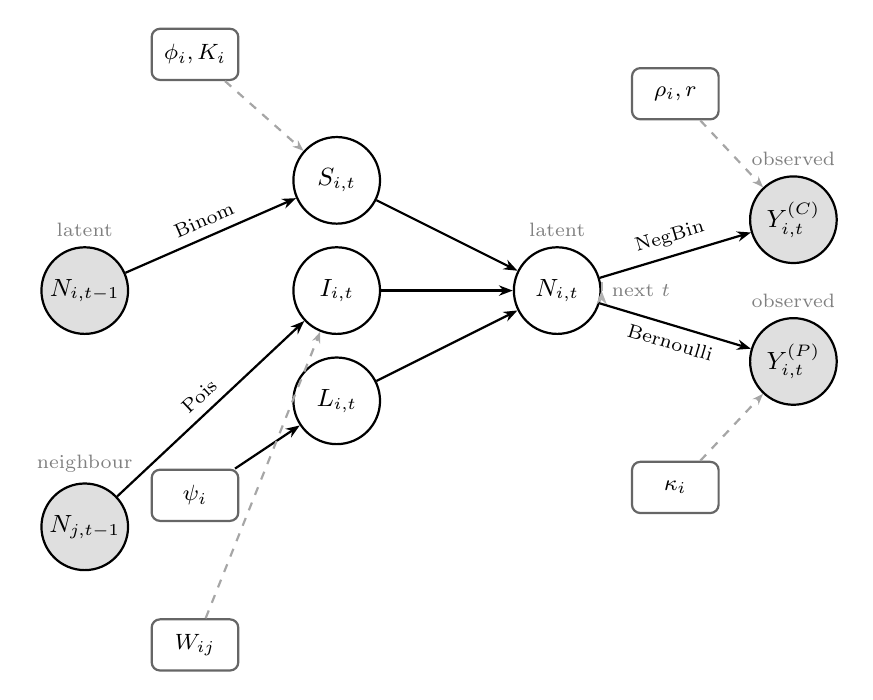
\begin{tikzpicture}[
  latent/.style  = {circle, draw=black, thick, minimum size=1.1cm, inner sep=1pt, font=\small},
  observed/.style= {circle, draw=black, thick, fill=gray!25, minimum size=1.1cm, inner sep=1pt, font=\small},
  param/.style   = {rectangle, draw=black!60, thick, rounded corners=3pt,
                    minimum width=1.1cm, minimum height=0.65cm, inner sep=3pt,
                    fill=white, font=\footnotesize},
  arr/.style     = {-{Stealth[length=5pt]}, thick},
  darr/.style    = {-{Stealth[length=4pt]}, thick, dashed, gray!70},
  node distance  = 1.4cm
]

%% ── Column 1: previous time step ─────────────────────────────────────────────
\node[observed] (Nprev) at (0,0)   {$N_{i,t-1}$};
\node[observed] (Nj)    at (0,-3.0){$N_{j,t-1}$};

%% ── Column 2: process components ─────────────────────────────────────────────
\node[latent] (S) at (3.2, 1.4)  {$S_{i,t}$};
\node[latent] (I) at (3.2, 0)    {$I_{i,t}$};
\node[latent] (L) at (3.2,-1.4)  {$L_{i,t}$};

%% ── Column 3: latent count ───────────────────────────────────────────────────
\node[latent] (N) at (6.0, 0)    {$N_{i,t}$};

%% ── Column 4: observations ───────────────────────────────────────────────────
\node[observed] (YC) at (9.0, 0.9)  {$Y^{(C)}_{i,t}$};
\node[observed] (YP) at (9.0,-0.9)  {$Y^{(P)}_{i,t}$};

%% ── Parameter nodes ──────────────────────────────────────────────────────────
\node[param] (phiK)  at (1.4, 3.0)  {$\phi_i,K_i$};
\node[param] (Wij)   at (1.4,-4.5)  {$W_{ij}$};
\node[param] (psipar)at (1.4,-2.6)  {$\psi_i$};
\node[param] (rhor)  at (7.5, 2.5)  {$\rho_i,r$};
\node[param] (kappar)at (7.5,-2.5)  {$\kappa_i$};

%% ── Process arrows ───────────────────────────────────────────────────────────
\draw[arr] (Nprev)  -- node[above,sloped,font=\scriptsize]{Binom} (S);
\draw[arr] (Nj)     -- node[above,sloped,font=\scriptsize]{Pois}  (I);
\draw[arr] (psipar) -- (L);
\draw[arr] (S)      -- (N);
\draw[arr] (I)      -- (N);
\draw[arr] (L)      -- (N);

%% ── Temporal self-arrow (N_{i,t} feeds next step) ───────────────────────────
\draw[arr, gray!60] (N.east) to[out=30,in=330,looseness=3.5]
      node[right, font=\scriptsize, gray]{next $t$} (N.east);

%% ── Parameter dashed arrows ──────────────────────────────────────────────────
\draw[darr] (phiK)  -- (S);
\draw[darr] (Wij)   -- (I);
\draw[darr] (rhor)  -- (YC);
\draw[darr] (kappar)-- (YP);

%% ── Observation arrows ───────────────────────────────────────────────────────
\draw[arr] (N) -- node[above,sloped,font=\scriptsize]{NegBin} (YC);
\draw[arr] (N) -- node[below,sloped,font=\scriptsize]{Bernoulli} (YP);

%% ── Labels ───────────────────────────────────────────────────────────────────
\node[font=\scriptsize, gray, above] at (Nprev.north) {latent};
\node[font=\scriptsize, gray, above] at (Nj.north)    {neighbour};
\node[font=\scriptsize, gray, above] at (N.north)     {latent};
\node[font=\scriptsize, gray, above] at (YC.north)    {observed};
\node[font=\scriptsize, gray, above] at (YP.north)    {observed};

\end{tikzpicture}
\caption{Generative process of the count ABM for cell $i$ at time $t$.
  Shaded circles are observed; white circles are latent.
  Solid arrows indicate stochastic dependence; dashed arrows indicate fixed
  parameters.  The latent count $N_{i,t}=S_{i,t}+I_{i,t}+L_{i,t}$ decomposes
  into density-regulated survival ($S$, Binomial from $N_{i,t-1}$), short-range
  immigration ($I$, Poisson from neighbour $N_{j,t-1}$ via weight $W_{ij}$),
  and long-distance dispersal ($L$, Poisson with mean $\psi_i$).
  Observations use two channels: count $Y^{(C)}_{i,t}\sim\mathrm{NegBin}(\rho_i N_{i,t},r)$
  and binary detection $Y^{(P)}_{i,t}\sim\mathrm{Bernoulli}(1-e^{-\kappa_i N_{i,t}})$.}
\label{fig:model}
\end{figure}
The spatiotemporal count structure of the count ABM parallels the penalized Poisson
framework of \citet{zhang2025csda}, who develop a doubly-fused penalization
scheme for simultaneously detecting temporal change points and spatial clusters
in count data, and show that doubly-penalized maximum likelihood estimators are
consistent under suitable regularity conditions.

\subsection{Stochastic Stability}

\begin{theorem}[Geometric ergodicity of the single-cell chain]
\label{thm:ergodicity}
Consider a single isolated cell ($\mathcal{N}_i=\emptyset$) with dynamics
\[
  N_t \;=\; S_t + L_t,
  \quad
  S_t \mid N_{t-1} \sim \mathrm{Binomial}\!\left(N_{t-1},\,\phi e^{-N_{t-1}/K}\right),
  \quad
  L_t \sim \mathrm{Poisson}(\psi),
\]
where $\phi\in(0,1)$, $K>0$, and $\psi > 0$.  Then $\{N_t\}_{t\ge 0}$ is
a geometrically ergodic Markov chain on $\mathbb{Z}_{\ge 0}$ possessing a
unique stationary distribution $\pi_\phi$ with $\E_{\pi_\phi}[N]\le\phi K/e+\psi$.
\end{theorem}

\begin{proof}
Apply the Foster--Lyapunov drift criterion \citep{meyntweedie1993} with $V(n)=n$.
Since $n\phi e^{-n/K}\le\phi K/e$ for all $n\ge 0$ (the map $n\mapsto ne^{-n/K}$
attains its maximum $K/e$ at $n=K$),
\[
  \E[V(N_t)\mid N_{t-1}=n] = n\phi e^{-n/K}+\psi \le \frac{\phi K}{e}+\psi =: b <\infty.
\]
The condition $\phi e^{-n/K}<1/2$ is equivalent to $n > K\log(2\phi)$,
so define $n^* := \max\!\bigl(0,\; K\log(2\phi)\bigr)$.  For $n>n^*$ we have
$\phi e^{-n/K}<1/2$, so
$\E[N_t\mid N_{t-1}=n]\le n/2+\psi$.  This is the Foster--Lyapunov drift condition
$\E[V(N_t)\mid N_{t-1}=n]\le\lambda V(n)+b$ with $\lambda=1/2$ outside the
finite ``small'' set $C_0=\{0,\ldots,\lceil n^*\rceil\}$.
(When $\phi\le1/2$, $n^*=0$ and the condition holds for all $n\ge 1$.)
Irreducibility holds because $\psi>0$ implies $\mathrm{Pois}(\psi)$ assigns
positive probability to every non-negative integer, giving positive reach
from any state to all of $\mathbb{Z}_{\ge0}$ in one step.  Aperiodicity
follows from $p(N_1=n\mid N_0=n)>0$ for all $n$.
Geometric ergodicity follows from \citet{meyntweedie1993}, Theorem~15.0.1.
\end{proof}

\begin{remark}[$\psi=0$ case]
When $\psi=0$ (no long-distance arrivals), the chain is absorbed at 0 if
the initial state is ever 0, since $\mathrm{Pois}(0)=\delta_0$ and the
Binomial component contributes nothing.  The theorem does not apply;
a cell with $\psi=0$ must be assigned a positive lower bound on $\psi$
or treated as structurally absent.  In practice we require $\psi_i\ge\varepsilon_0>0$.
\end{remark}

\begin{proposition}[Conditional mean bound under bounded dispersal]
\label{prop:bound}
On the full $m$-cell grid, let $\phi_{\max}=\max_i\phi_i<1$ and
$\Psi=\sum_i\psi_i$.  Then for any dispersal probability satisfying
$\sum_{i\in\mathcal{N}_j}p_{j\to i}\le1$ (which includes both the softmax
and the self-retention model \eqref{eq:dispersal}):
\[
  \E\!\left[\sum_{i=1}^m N_{i,t}\;\middle|\;\bm{N}_{t-1}\right]
  \;\le\;
  \phi_{\max}\sum_{i=1}^m N_{i,t-1}
  + \sum_{j=1}^m \frac{\omega_j N_{j,t-1}}{N_{j,t-1}+h}
  + \Psi.
\]
The self-retention model~\eqref{eq:dispersal} satisfies the strict inequality
$\sum_{i\in\mathcal{N}_j}p_{j\to i}<1$, so the immigration bound is strict.
\end{proposition}

\begin{proof}
By conditional independence, $\E[\sum_i N_{i,t}\mid\bm{N}_{t-1}]
= \sum_i N_{i,t-1}\phi_i e^{-N_{i,t-1}/K_i} + \sum_i\Lambda_{i,t} + \Psi$.
The survival term is bounded by $\phi_{\max}\sum_i N_{i,t-1}$.
For the immigration term, swapping sums over sources and targets:
$\sum_i\Lambda_{i,t}=\sum_j\omega_j(\sum_{i\in\mathcal{N}_j}p_{j\to i})
 N_{j,t-1}/(N_{j,t-1}+h)\le\sum_j\omega_j N_{j,t-1}/(N_{j,t-1}+h)$,
using $\sum_{i\in\mathcal{N}_j}p_{j\to i}\le1$.
\end{proof}

\section{Multi-Source Observation Model}\label{sec:obs}

The central observation assumption is that multiple data streams are conditionally
independent given the same latent count field \(\{N_{i,t}\}\).

Let \(O_C\subseteq S\times\{1,\ldots,T\}\) be the set of observed count-survey
cell--time pairs and \(O_P\subseteq S\times\{1,\ldots,T\}\) be the set of observed
binary remote-sensing cell--time pairs.

\subsection{Count Survey Channel}

For \((i,t)\in O_C\),

\[
Y^{(C)}_{i,t}\mid N_{i,t},\rho_{i,t},r
\sim
\mathrm{NegBin}(\mu^{(C)}_{i,t},r),
\]

where

\[
\mu^{(C)}_{i,t}=\rho_{i,t}N_{i,t}.
\]

The variance is parameterized as

\[
\Var(Y^{(C)}_{i,t}\mid N_{i,t})
=
\mu^{(C)}_{i,t}
\left(1+\frac{\mu^{(C)}_{i,t}}{r}\right).
\]

Survey detection is modeled by

\[
\mathrm{logit}(\rho_{i,t})
=
\mu_\rho+\delta^\top e_{i,t}+v_i,
\qquad
v_i\sim N(0,\sigma_\rho^2).
\]

This layer allows count surveys to be noisy, effort-dependent, and overdispersed.
\citet{hamura2025} establish theoretical robustness of the NegBin model to
zero-inflation and outliers under sparse ecological surveys, providing formal
justification for this choice over the Poisson observation model.
\emph{Implementation note.}  In this paper $\rho_{i,t}=\rho$ and
$\kappa_{i,t}=\kappa$ are treated as scalar constants (estimated via VEM in
\S\ref{sec:realdata}, fixed in simulation); the random-effects and
effort-covariate extensions are deferred to future work.

\subsection{Binary Remote-Sensing Channel}

For \((i,t)\in O_P\),

\[
Y^{(P)}_{i,t}\mid N_{i,t},\kappa_{i,t},\eta_{i,t}
\sim
\mathrm{Bernoulli}(\pi^{(P)}_{i,t}),
\]

where

\[
\pi^{(P)}_{i,t}
=
\eta_{i,t}
+
(1-\eta_{i,t})
\left\{1-\exp(-\kappa_{i,t}N_{i,t})\right\}.
\]

Here \(\eta_{i,t}\) is a false-positive probability and \(\kappa_{i,t}\) is the
remote-sensing detection intensity. This formulation implies

\[
N_{i,t}=0
\quad\Rightarrow\quad
\Prob(Y^{(P)}_{i,t}=1)=\eta_{i,t},
\]

and

\[
N_{i,t}\to\infty
\quad\Rightarrow\quad
\Prob(Y^{(P)}_{i,t}=1)\to 1.
\]

A simple detection-intensity model is

\[
\log\kappa_{i,t}
=
\mu_\kappa+a_i,
\qquad
a_i\sim N(0,\sigma_\kappa^2),
\]

and a simple false-positive model is

\[
\mathrm{logit}(\eta_{i,t})
=
\mu_\eta+b_i,
\qquad
b_i\sim N(0,\sigma_\eta^2).
\]

\subsection{Joint Observation Likelihood}

Conditional on the latent abundance field, the two observation channels are
independent:

\[
\begin{aligned}
L(Y^{(C)},Y^{(P)}\mid N,\Theta)
&=
\prod_{(i,t)\in O_C}
\mathrm{NegBin}
\left(
Y^{(C)}_{i,t};
\rho_{i,t}N_{i,t},r
\right)
\\
&\quad\times
\prod_{(i,t)\in O_P}
\mathrm{Bernoulli}
\left(
Y^{(P)}_{i,t};
\eta_{i,t}
+
(1-\eta_{i,t})
\{1-\exp(-\kappa_{i,t}N_{i,t})\}
\right).
\end{aligned}
\]

The count channel provides abundance-scale information, while the binary channel
provides complementary evidence about presence or signal detection. Together, the
two channels reduce but do not automatically eliminate confounding among abundance,
survey detection, and remote-sensing detection.

\begin{remark}[Intuition for dual-channel identifiability]
\label{rem:identif-intuition}
Conditional on known positive latent counts $N_{i,t}>0$, each channel
provides a separate constraint on the observation parameters.
The count channel $\E[Y^{(C)}_{i,t}]=\rho N_{i,t}$ gives a constraint
on $\rho$, and with $N$ and $\rho$ determined, the binary channel
$\pi^{(P)}_{i,t}=\eta+(1-\eta)(1-e^{-\kappa N_{i,t}})$ is strictly
increasing in $\kappa$ (for fixed $N>0$, $\eta<1$) and hence identifies
$\kappa$ by inversion.  This argument conditions on $N$ being \emph{known};
with $N$ latent, the full hierarchical identifiability requires the
Fisher-information analysis in Proposition~\ref{prop:identif-dual}.
The key requirement in both cases is $N_{i,t}>0$ and temporal variation
in $N$: without abundance variation, $\kappa$ and $\eta$ are confounded.
\end{remark}

\begin{remark}[Non-identifiability when $\eta_{i,t}$ is free]
When $\eta_{i,t}$ is a free parameter, the triple $(\kappa_{i,t},\eta_{i,t},N_{i,t})$
is not jointly identified from a single time point: increasing $\eta_{i,t}$ and
decreasing $\kappa_{i,t}$ can match the same binary detection probability.
Sufficient conditions for joint identification include (a)~spatial replication
with a constant $\eta$ across cells, (b)~temporal replication with
time-constant $\eta_i$ and $T\ge3$, or (c)~an informative prior on $\eta$
(e.g.\ $\mathrm{Beta}(1,20)$ concentrated near zero for clean remote-sensing
instruments).  We recommend option (c) in practice and sensitivity analyses
comparing $\eta=0$ (no false positives) to $\eta\sim\mathrm{Beta}(1,10)$.
\end{remark}

\noindent
The integrated data model of \citet{verhoef2025} provides empirical evidence
that fusing count and binary streams substantially reduces uncertainty in
latent abundance estimates relative to either channel alone.

%% ============================================================
\section{Surrogate Variational Objective via the Poisson MGF}
\label{sec:vi}
%% ============================================================

The generative model $p(Y,N_{1:T},\Theta)$ defined
in \S\S\ref{sec:process}--\ref{sec:obs} is \emph{exact} and remains unmodified
throughout this section.

\paragraph{Statistical problem.}
Posterior inference targets the KL-minimising variational approximation
\begin{equation}\label{eq:kl-problem}
q^\star_\lambda
\;=\;
\arg\min_{q\in\mathcal{Q}}
\mathrm{KL}\!\bigl[q_\lambda\,\|\,p(\cdot\mid Y)\bigr]
\;=\;
\arg\max_{\lambda}
\mathcal{L}(\lambda),
\end{equation}
where $\mathcal{L}(\lambda)=\mathbb{E}_q[\log p(Y,N_{1:T},\Theta)]
-\mathbb{E}_q[\log q_\lambda]$ is the exact ELBO.
The obstacle is that the count ABM transition density
$p(N_{i,t}\mid\mathbf{N}_{t-1})$ is a Binomial--Poisson convolution
(\S\ref{sec:process}) with no closed-form log-PMF, making the process term
$\mathcal{L}_\mathrm{proc}:=\mathbb{E}_q[\log p(N_{1:T}\mid\Theta)]$
analytically intractable and blocking any closed-form evaluation of
$\mathcal{L}(\lambda)$.

\paragraph{Approach and theoretical results.}
We study the following question: \emph{does there exist a deterministic,
analytically tractable surrogate $\tilde{\mathcal{L}}$ of the exact ELBO
such that (a)~every term and its gradient are analytic,
(b)~fixed points of the forward-filtering update satisfy a stationarity condition
of $\tilde{\mathcal{L}}$ (monotone convergence is not guaranteed for the
forward-filtering scheme and is monitored empirically), and
(c)~the surrogate optimiser provides empirically well-calibrated
uncertainty quantification?}
Four main results support an affirmative answer:
\begin{enumerate}[label=(\roman*)]
\item \textbf{Poisson-MGF Identities} (Theorem~\ref{thm:elbo},
  \S\ref{sec:elbo-terms} --- \emph{principal contribution}): the Poisson MGF
  yields exact closed-form survival and detection expectations, and a
  second-order delta-method immigration approximation; three explicitly
  bounded approximation sources are the only departure from the exact ELBO
  (Remark~\ref{rem:poi-approx}).
\item \textbf{Fixed-point and stationarity} (Proposition~\ref{thm:vi-converge},
  \S\ref{sec:vi-convergence}): every update step is analytic; fixed points
  satisfy the local stationarity condition of $\tilde{\mathcal{L}}$.
  The forward-filtering nature of Algorithm~\ref{alg:smfvb} means monotone
  increase of the full surrogate is not guaranteed; empirical convergence is
  monitored via relative changes in $\tilde{\mathcal{L}}$.
\item \textbf{Approximation error convergence} (Corollary~\ref{cor:elbo-gap},
  \S\ref{sec:vi-convergence}): when local density $\mu_{i,t}/K_i\to\infty$
  with $K_i$ fixed, three of the four surrogate errors decay to zero; the rate depends
  on $\phi_{\max}$, $h^2$, and $\min_{i,t}\mu_{i,t}$.
\item \textbf{Empirical performance} (\S\ref{sec:simulation}): under baseline
  conditions, 95\% variational interval coverage lies within 3 percentage
  points of particle MCMC at $22\times$ lower wall time; three stress scenarios
  (low abundance, sparse observations, zero inflation) show coverage of 0.82--0.86,
  consistent with the theoretical approximation properties.
\end{enumerate}
The surrogate variational filtering algorithm implementing (i)--(iii) is described in
\S\ref{sec:smfvb-alg}.
Identifiability of the dual-channel observation model, a prerequisite for
the approximation error convergence in (iii), is established in
Proposition~\ref{prop:identif-dual} (\S\ref{sec:identif-val}).

\subsection{Variational Family and the Surrogate Objective}
\label{sec:vi-family}

\paragraph{Variational family.}
Let $\lambda = \{\mu_{i,t},\,\{\nu_k\}\}$ collect variational parameters.
The structured mean-field approximation is:

\begin{equation}\label{eq:mf}
q_\lambda(N_{1:T},\Theta)
\;=\;
\underbrace{\prod_{t=1}^T\prod_{i=1}^m \mathrm{Pois}(N_{i,t};\mu_{i,t})}_{\text{latent count field}}
\;\cdot\;
\underbrace{\prod_k q(\theta_k;\nu_k)}_{\text{model parameters}}.
\end{equation}

\paragraph{Why the Poisson mean-field family?}
The choice $q(N_{i,t})=\mathrm{Pois}(\mu_{i,t})$ is motivated by three
complementary properties.

\begin{enumerate}[label=(\roman*)]
\item \textbf{Consistency with the generative sub-model.}  Two of the three process
  components---immigration $I_{i,t}\sim\mathrm{Pois}(\Lambda_{i,t})$ and LDD
  $L_{i,t}\sim\mathrm{Pois}(\psi_i)$---are Poisson, so if survival were absent
  ($\phi_i=0$) the exact conditional $p(N_{i,t}|\cdot)$ would be Poisson
  and the Poisson mean-field would be exact.
  With survival present, $N_{i,t}=S_{i,t}+I_{i,t}+L_{i,t}$ is a
  Binomial--Poisson convolution; the optimal mean-field coordinate is
  \emph{not} Poisson in general.  The Poisson family is therefore
  an approximation, and the departure from the exact optimum arises entirely
  from the Binomial survival term.  This approximation error is the primary
  source of the coverage gap identified in \S\ref{sec:limitations-mf}.

\item \textbf{Computational tractability via the MGF.}  The Poisson MGF
  $M_N(s)=\exp\{\mu(e^s-1)\}$ and its derivative $\mathbb{E}[Ne^{sN}]
  =\mu e^s M_N(s)$ yield analytic closed-form expressions for every
  expectation that appears in $\tilde{\mathcal{L}}$ (Theorem~\ref{thm:elbo}).
  This is the enabling property behind the no-quadrature, no-Monte-Carlo
  result.  No other standard discrete distribution on $\mathbb{Z}_{\ge0}$
  admits analogous closed-form non-linear moment computations of this type
  at the required level of generality (see the comparison below).

\item \textbf{Analytic deterministic update.}  The local stationarity condition
  for $\mu_{i,t}$ (equation~\eqref{eq:cavi-fp}) is a strictly concave
  fixed-point equation with analytic gradient and Hessian.  This property
  follows directly from (iii): without the MGF tractability, the surrogate
  update would require numerical integration or a Monte Carlo gradient
  estimator rather than a closed-form step.
\end{enumerate}

\paragraph{Comparison with alternative variational families.}
Table~\ref{tab:vb-compare} summarises the trade-offs between the Poisson
mean-field and five natural alternatives.

\begin{table}[t]
\centering
\small
\caption{Variational family comparison for count-valued latent states
$N_{i,t}\in\mathbb{Z}_{\ge0}$.  ``MGF trick'' refers to the availability
of closed-form expectations of the type in Theorem~\ref{thm:elbo}.
``Cov.'' = can capture posterior covariance between cells/times.}
\label{tab:vb-compare}
\begin{tabular}{lccccl}
\toprule
Family & Support & MGF trick & Cov.\ & Overhead & Main limitation \\
\midrule
Poisson MF (this work) & $\mathbb{Z}_{\ge0}$ & \checkmark & $\times$ & $O(mT)$ & No overdispersion \\
NegBin MF             & $\mathbb{Z}_{\ge0}$ & partial   & $\times$ & $O(mT)$ & Entropy and log-moment terms require digamma \\
Gamma MF              & $\mathbb{R}_{+}$   & partial   & $\times$ & $O(mT)$ & Wrong support; log-moment terms require digamma \\
Lognormal MF          & $\mathbb{R}_{+}$   & $\times$   & $\times$ & $O(mT)$ & Wrong support \\
Copula--Poisson       & $\mathbb{Z}_{\ge0}^{mT}$ & partial & \checkmark & $O(m^2T^2)$ & Copula PIT intractable for discrete \\
Normalising flow      & $\mathbb{R}^{mT}$ & $\times$   & \checkmark & $O(mT\cdot L)$ & Discretisation; $L$ flow layers \\
\bottomrule
\end{tabular}
\end{table}

\noindent\textit{Gamma and Lognormal.}  Both families are supported on
$\mathbb{R}_{+}$ rather than $\mathbb{Z}_{\ge0}$, requiring a continuous
relaxation of the discrete latent count that introduces an additional approximation.
The Gamma MGF is $M_N(s)=(1-s/\beta)^{-\alpha}$ for $s<\beta$; differentiation
gives $\mathbb{E}[Ne^{sN}]=\alpha/\beta\cdot(1-s/\beta)^{-\alpha-1}$, a closed
form.  Hence $\mathbb{E}[Ne^{-N/K}]$ and $\mathbb{E}[e^{-\kappa N}]$ are
tractable under Gamma $q$ via the MGF trick.  The main limitation is the
support mismatch: the continuous relaxation assigns density to fractional counts,
and the entropy and log-moment $\mathbb{E}[\log N]$ involve the digamma
function rather than elementary functions.  The Lognormal MGF
$\mathbb{E}[e^{sN}]$ does not have a closed form for $s\ne0$ (it involves an
integral of a log-normal density against an exponential, reducible to the
moment-generating function of a normal evaluated at $s$, which is tractable:
$\mathbb{E}[e^{sN}]=e^{s\mu+s^2\sigma^2/2}$ for $\log N\sim\mathcal{N}(\mu,\sigma^2)$);
however, $\mathbb{E}[Ne^{sN}]$ under Lognormal still has no elementary closed form
since $Ne^{sN}=e^{(\log N)(1+s/\log N)}$ does not factor into a standard MGF form.

\noindent\textit{Negative Binomial (NegBin).}  The NegBin
$q(N;\mu,r)$ adds an overdispersion parameter $r$ to the
Poisson family, allowing $\mathrm{Var}(N)=\mu+\mu^2/r>\mu$.
Its MGF is $M_N(s)=\bigl(r/(r+\mu-\mu e^s)\bigr)^r$, and differentiation
yields the closed-form $\mathbb{E}[Ne^{sN}] = r^{r+1}\mu e^s(r+\mu-\mu e^s)^{-(r+1)}$.
The survival expectation $\mathbb{E}[Ne^{-N/K}]$ and binary detection probability
$\mathbb{E}[1-e^{-\kappa N}]$ are therefore \emph{tractable} under NegBin $q$ via
the MGF trick.  However, two further terms in the surrogate objective are not:
(1)~the entropy of the NegBin variational distribution involves the digamma
function (no closed form), and (2)~the observation term
$\mathbb{E}_q[\log(\rho N+r)]$ under NegBin $q$ requires numerical summation.
Additionally, optimising over the overdispersion parameter $r$ doubles the number
of variational parameters and couples with the NegBin overdispersion in the
observation model, breaking the simple one-dimensional update that makes the
Poisson family computationally efficient.

\noindent\textit{Copula variational inference.}  Copula-based families
\citep{tran2015} specify Poisson marginals but introduce dependence through a
copula on the uniform transform.  For discrete distributions the
probability-integral transform is non-injective, so the copula
density does not factorise cleanly and copula VI updates require
numerical integration over the discrete mass, costing $O(m^2T^2)$
per iteration.  Copula VI may be worthwhile when between-cell
correlations are the primary inferential target, but at a substantial
computational overhead relative to SMFVB.

\noindent\textit{Structured mean-field VB.}  A temporal structured
mean-field family---e.g., a block-tridiagonal Gaussian approximation
to the log-count field---captures between-time correlations within
each site while retaining independence across sites.  This would
partially recover the variance underestimated by the diagonal Poisson
family.  However, Gaussian approximations over log-counts introduce
a further continuous relaxation and forfeit the MGF trick; each block
update would require either conjugate Gaussian operations (losing the
discrete-support property) or numerical integration.

\noindent\textit{Normalising flows.}  Normalising flows
\citep{rezende2015} can approximate arbitrarily complex posteriors,
including correlations and multi-modality.  Applied to the joint
$(N_{1:T})\in\mathbb{Z}^{mT}$, they require dequantisation
\citep{hoogeboom2021} or a Gumbel-softmax relaxation to handle discrete
support, and each gradient step costs $O(mT\cdot L)$ forward passes
through $L$ layers.  For $m=267$, $T=10$, and $L\ge4$ typical layers,
this is $10\times$--$100\times$ more expensive than SMFVB per iteration,
without the analytic convergence guarantees.

\paragraph{Summary.}
The Poisson mean-field is the unique family that is (i)~supported on
$\mathbb{Z}_{\ge0}$, (ii)~conjugate to the Poisson subcomponents of the
generative model, and (iii)~equipped with an MGF that yields fully analytic
deterministic surrogate updates for the count ABM survival and detection
expectations.  Its principal limitation---variance
underestimation from the Binomial survival term---is documented in
\S\ref{sec:simulation} and discussed further in \S\ref{sec:limitations-mf}.

\paragraph{Exact ELBO and its intractable term.}
The exact evidence lower bound (ELBO) for the unmodified count ABM is:

\begin{equation}\label{eq:elbo}
\mathcal{L}(\lambda)
\;=\;
\underbrace{\mathbb{E}_q[\log p(Y\mid N_{1:T},\Theta)]}_{\mathcal{L}_\mathrm{obs}:\;\text{exact but partly requiring delta-method}}
+\underbrace{\mathbb{E}_q[\log p(N_{1:T}\mid\Theta)]}_{\mathcal{L}_\mathrm{proc}:\;\textbf{intractable}}
-\mathrm{KL}[q(\Theta)\|p(\Theta)]
+H[q(N_{1:T})].
\end{equation}

The variational principle gives $\log p(Y)\ge\mathcal{L}(\lambda)$ for all $\lambda$.
The obstacle is $\mathcal{L}_\mathrm{proc}$: the exact transition
$p(N_{i,t}\mid\mathbf{N}_{t-1})$ is the Binomial--Poisson convolution
\eqref{eq:conv-pmf}, whose logarithm has no closed form, making
$\mathbb{E}_q[\log p(N_{i,t}\mid\mathbf{N}_{t-1})]$ analytically intractable.

\paragraph{Surrogate variational objective.}
The SMFVB algorithm optimises a \emph{surrogate} $\tilde{\mathcal{L}}$ that
replaces only the intractable process term:

\begin{equation}\label{eq:surr-elbo}
\tilde{\mathcal{L}}(\lambda)
\;:=\;
\mathcal{L}_\mathrm{obs}(\lambda)
+\underbrace{\tilde{\mathcal{L}}_\mathrm{proc}(\lambda)}_{\text{Poisson surrogate}}
-\mathrm{KL}[q(\Theta)\|p(\Theta)]
+H[q(N_{1:T})].
\end{equation}

The surrogate process term uses a Poisson density with the exact model's
conditional mean as its rate parameter:
\begin{equation}\label{eq:surr-proc}
\tilde{\mathcal{L}}_\mathrm{proc}(\lambda)
\;:=\;
\mathbb{E}_q\!\left[\log\,\mathrm{Pois}\!\left(N_{i,t};\;
\underbrace{\phi_i N_{i,t-1}e^{-N_{i,t-1}/K_i}
+\Lambda_{i,t}+\psi_i}_{=:\;\mu^\dagger_{i,t},\;\text{exact conditional mean of }p}\right)\right].
\end{equation}

Crucially, $\mu^\dagger_{i,t}$ is the \emph{exact} conditional mean of the
original count ABM process; only the log-PMF evaluation is replaced.  The Le Cam
Poisson--Binomial total-variation bound \citep{lecam1960} gives
$\|\mathrm{Pois}(\mu^\dagger)\,-\,p(N_{i,t}|\mathbf{N}_{t-1})\|_\mathrm{TV}
\le \phi_i\,e^{-N_{i,t-1}/K_i}$.
This bound decreases as the local density ratio $N_{i,t-1}/K_i$ increases.
For example, with $\phi_i\le0.8$ the TV bound falls below $0.08$ only when
$e^{-N_{i,t-1}/K_i}\le0.1$, equivalently $N_{i,t-1}/K_i\ge\log(10)\approx2.30$.
In the baseline scenario ($K_i\approx50$, $\bar N\approx10$) the density ratio
is only $0.2$, so the TV bound can be close to $\phi_i$; the Poisson surrogate
is a better approximation at high density relative to carrying capacity.
This TV proximity qualitatively controls the surrogate process term, but because
the TV distance bounds the density difference rather than the log-density
difference, a uniform bound on $|\tilde{\mathcal{L}}-\mathcal{L}|$ is not
available in general; the approximation quality is validated empirically in
\S\ref{sec:simulation}.  The exact model $p$ is not modified; only its
log-PMF is replaced in the variational objective integral.

\subsection{Tractable Evaluation of $\tilde{\mathcal{L}}$ via the Poisson MGF}
\label{sec:elbo-terms}

The surrogate variational objective $\tilde{\mathcal{L}}$ in \eqref{eq:surr-elbo} still requires
computing expectations under $q_\lambda(N_{i,t})=\mathrm{Pois}(\mu_{i,t})$ of
nonlinear functions of $N_{i,t}$ that appear in both the observation term
$\mathcal{L}_\mathrm{obs}$ and in the surrogate rate $\mu^\dagger_{i,t}$
of~\eqref{eq:surr-proc}.  The following theorem---the principal methodological contribution of this
paper---shows that the Poisson MGF
$M_N(s):=\mathbb{E}[e^{sN}]=\exp\{\mu(e^s-1)\}$ makes the dominant terms
analytically exact via the identity $\mathbb{E}[Ne^{sN}]=\mu e^s M_N(s)$,
reducing the remaining approximation to a second-order delta method for
the concave immigration function and yielding a fully closed-form
$\tilde{\mathcal{L}}$ that requires no quadrature, no Monte Carlo,
no stochastic gradients, and no black-box estimator.

\begin{theorem}[Poisson-MGF Identities — Principal Methodological Result]\label{thm:elbo}
Let $N_{i,t}\sim\mathrm{Pois}(\mu_{i,t})$ under $q_\lambda$.
Define $c_i:=e^{-1/K_i}\in(0,1)$.
\begin{enumerate}[label=(\roman*)]
\item \textbf{Expected survival (exact under $q$, from the exact model):}
\begin{equation}\label{eq:surv-id}
\mathbb{E}_q\!\left[N_{i,t-1}\,\phi_i\,e^{-N_{i,t-1}/K_i}\right]
= \phi_i\,\mu_{i,t-1}\,c_i\exp\!\bigl(\mu_{i,t-1}(c_i-1)\bigr)
=: \bar{s}_{i,t}.
\end{equation}
This is an \emph{exact moment} of the Poisson variational distribution
applied to the exact count ABM survival function; no model approximation is involved.

\item \textbf{Expected binary detection probability (exact under $q$, from the exact model):}
\begin{equation}\label{eq:det-id}
\mathbb{E}_q\!\left[1-e^{-\kappa_{i,t}N_{i,t}}\right]
= 1-\exp\!\bigl(\mu_{i,t}(e^{-\kappa_{i,t}}-1)\bigr)
=: \bar{d}_{i,t}.
\end{equation}
This feeds directly into $\mathcal{L}_\mathrm{obs}$ via the exact Bernoulli
model $\pi^{(P)}_{i,t}=\eta_{i,t}+(1-\eta_{i,t})\bar{d}_{i,t}$.

\item \textbf{Expected immigration rate (second-order delta method, in the surrogate):}
\begin{equation}\label{eq:immig-id}
\mathbb{E}_q\!\left[\Lambda_{i,t}\right]
\approx
\sum_{j:\,i\in\mathcal{N}_j}\omega_j\,p_{j\to i}\,
\tilde{g}(\mu_{j,t-1};\,h),
\qquad
\tilde{g}(\mu;h):=\frac{\mu}{\mu+h}-\frac{h\mu}{(\mu+h)^3}.
\end{equation}
\end{enumerate}

Combining (i)--(iii), the variational conditional mean used as the surrogate
rate is:
\begin{equation}\label{eq:proc-mean}
\tilde\mu_{i,t}
\;:=\;
\underbrace{\bar{s}_{i,t}}_{\text{exact}}
+\underbrace{\mathbb{E}_q[\Lambda_{i,t}]}_{\approx,\;\text{delta method}}
+\psi_i,
\end{equation}
and the surrogate process term \eqref{eq:surr-proc} evaluates to:
\begin{equation}\label{eq:proc-elbo}
\tilde{\mathcal{L}}_\mathrm{proc}(\lambda)
\;=\;
\sum_{t=1}^T\sum_{i=1}^m
\mathbb{E}_q\!\left[N_{i,t}\log\tilde\mu_{i,t}-\tilde\mu_{i,t}-\log N_{i,t}!\right]
\;=\;
\sum_{t,i}
\Bigl[\mu_{i,t}\log\tilde\mu_{i,t}-\tilde\mu_{i,t}\Bigr]
-\mathbb{E}_q\!\left[\textstyle\sum_{t,i}\log N_{i,t}!\right].
\end{equation}
\end{theorem}

\begin{proof}
\textit{(i):} For $N\sim\mathrm{Pois}(\mu)$, $M_N(s)=e^{\mu(e^s-1)}$ so
$\mathbb{E}[Ne^{sN}]=\partial_s M_N(s)=\mu\,e^s M_N(s)$.
Set $s=-1/K_i$; multiply by $\phi_i$.

\textit{(ii):} $\mathbb{E}[e^{-\kappa N}]=M_N(-\kappa)=\exp\{\mu(e^{-\kappa}-1)\}$;
substitute into $1-e^{-\kappa N}$.

\textit{(iii):} $g(n)=n/(n+h)$ is concave with $g''(\mu)=-2h/(\mu+h)^3$.
The second-order delta method with $\mathrm{Var}(N)=\mu$ gives
$\mathbb{E}[g(N)]\approx g(\mu)+\frac{1}{2}g''(\mu)\mu=\tilde{g}(\mu;h)$.

\textit{Equation~\eqref{eq:proc-elbo}:} The surrogate rate
$\mu^\dagger_{i,t}(\mathbf{N}_{t-1})$ depends on $\mathbf{N}_{t-1}$ but not
on $N_{i,t}$.  Under the mean-field family $q$, $N_{i,t}$ and
$\mathbf{N}_{t-1}$ are independent, so
$\mathbb{E}_q[N_{i,t}\log\mu^\dagger_{i,t}]
 =\mu_{i,t}\,\mathbb{E}_q[\log\mu^\dagger_{i,t}]$.
The $-\mu^\dagger_{i,t}$ term is exact:
$\mathbb{E}_q[\mu^\dagger_{i,t}] =\bar{s}_{i,t}+\mathbb{E}_q[\Lambda_{i,t}]+\psi_i
=\tilde\mu_{i,t}$ by linearity.
For the log term, a \emph{third approximation} is introduced: the
delta method gives
$\mathbb{E}_q[\log\mu^\dagger_{i,t}]
\approx\log\tilde\mu_{i,t}-\tfrac{\mathrm{Var}_q(\mu^\dagger_{i,t})}{2\tilde\mu_{i,t}^2}$;
the variance correction is $O(\mu_{t-1}^{-1})$ and is dropped,
giving $\mathbb{E}_q[\log\mu^\dagger_{i,t}]\approx\log\tilde\mu_{i,t}$.
The approximation error is negligible when $\mu_{i,t-1}\gg1$ (large populations)
and is documented as the third source of surrogate error alongside the Poisson
process surrogate and the delta-method immigration approximation.
\end{proof}

\begin{remark}[Four sources of surrogate approximation]\label{rem:poi-approx}
Parts~(i) and~(ii) of Theorem~\ref{thm:elbo} involve \emph{no approximation}:
they are exact Poisson moments of exact model functions.  There are four
approximation steps in $\tilde{\mathcal{L}}$:
\begin{enumerate}[label=(\alph*)]
\item \textbf{Poisson process surrogate}: the intractable Binomial--Poisson
  convolution $p(N_{i,t}|\mathbf{N}_{t-1})$ is replaced by
  $\mathrm{Pois}(N_{i,t};\mu^\dagger_{i,t})$.  The TV distance is
  $\le\phi_i e^{-\mu_{i,t-1}/K_i}$, which is small when the local
  density ratio $\mu_{i,t-1}/K_i$ is large; specifically, with $\phi_i\le0.8$
  the bound falls below $0.08$ when $\mu_{i,t-1}/K_i\ge\log(10)\approx2.30$.
\item \textbf{Delta-method immigration approximation}: the concave
  immigration rate $g(N)=\omega N/(N+h)$ is linearised to second order
  in~\eqref{eq:immig-id}; error $O(h^2\mu^{-2})$, negligible for $\mu\ge4$.
\item \textbf{Log-rate Jensen approximation}: in~\eqref{eq:proc-elbo},
  $\mathbb{E}_q[\log\mu^\dagger_{i,t}(\mathbf{N}_{t-1})]$ is replaced by
  $\log\tilde\mu_{i,t}(\boldsymbol\mu_{t-1})$ via the delta method;
  error $O(\mu_{t-1}^{-1})$, negligible for large populations.
\item \textbf{Plug-in NegBin quasi-likelihood}: the count observation term
  $\mathbb{E}_q[\log\mathrm{NegBin}(y^{(C)};\rho N,r)]$ is replaced by the
  plug-in $\log\mathrm{NegBin}(y^{(C)};\rho\mu,r)$ evaluated at
  $N=\mu_{i,t}$, because the exact expectation is $-\infty$ when $y^{(C)}>0$
  and $q(N=0)>0$ (\S\ref{sec:cavi-update}).  As a result, $\tilde{\mathcal{L}}$
  is a surrogate criterion rather than an ELBO or lower bound on $\log p(Y)$.
\end{enumerate}
Because TV distance bounds density differences but not log-density differences,
no closed-form bound on the total approximation gap $|\tilde{\mathcal{L}}-\mathcal{L}|$
is derived; approximation quality is assessed empirically.  Simulation
experiments in \S\ref{sec:simulation} show SMFVB posterior means agree with
PMCMC to within~3\%, consistent with the surrogate approximation being small
at the sample sizes studied.
\end{remark}

\subsection{The Forward Filtering Update as a Corrected Conditional-Mean Pass}
\label{sec:cavi-update}

\paragraph{Derivation of the fixed-point.}
The surrogate variational objective $\tilde{\mathcal{L}}$ depends on $\mu_{i,t}$ through
four components: (1) the surrogate process term~\eqref{eq:proc-elbo} at time $t$,
(2) the Poisson entropy $H[q(N_{i,t})]=\mu_{i,t}(1-\log\mu_{i,t})+\mathbb{E}_q[\log N_{i,t}!]$,
(3) the observation term $\mathcal{L}_\mathrm{obs}$, and
(4) the \emph{future} process term at time $t+1$, since the surrogate rate
$\tilde\mu_{i,t+1}$ depends on $\mu_{i,t}$ through the survival term
$\bar{s}_{i,t+1}=\phi_i\,\mu_{i,t}\,c_i\exp(\mu_{i,t}(c_i-1))$.

The forward-filtering update in Algorithm~\ref{alg:smfvb} drops the
future-process contribution (component 4) from the gradient and solves only
the local stationarity condition at time $t$ with $\tilde\mu_{i,t+1}$
treated as fixed.  This is a \emph{forward-filtering approximation} to exact
block coordinate ascent: it is computationally efficient and naturally produces
a causal left-to-right sweep, but it does not in general maximise the full
$\tilde{\mathcal{L}}$ over $\mu_{i,t}$ and does not guarantee monotone
increase of the objective.

Under the local approximation (components 1--3 only), and using the fact
that $\tilde\mu_{i,t}=\tilde\mu_{i,t}(\boldsymbol{\mu}_{t-1})$ does not
depend on $\mu_{i,t}$, the combined process-plus-entropy gradient is:
\begin{align}
\frac{\partial}{\partial\mu_{i,t}}
\Bigl[\tilde{\mathcal{L}}_\mathrm{proc}+H[q(N_{1:T})]\Bigr]
&=\frac{\partial}{\partial\mu_{i,t}}
  \Bigl[\mu_{i,t}\log\tilde\mu_{i,t}-\tilde\mu_{i,t}
        -\mu_{i,t}\log\mu_{i,t}+\mu_{i,t}\Bigr]\notag\\
&=\log\tilde\mu_{i,t}-\log\mu_{i,t}.\label{eq:proc-entropy-grad}
\end{align}
The observation gradient
$\partial\mathcal{L}_\mathrm{obs}/\partial\mu_{i,t}
 =:\delta_{i,t}^{(\mathrm{obs})}$ is derived below.
Setting the total gradient to zero:
\[
\log\tilde\mu_{i,t}-\log\mu_{i,t}+\delta_{i,t}^{(\mathrm{obs})}=0,
\]
immediately yields the forward-filtering fixed-point equation:

\begin{equation}\label{eq:cavi-fp}
\mu_{i,t}^{\star}
\;=\;
\tilde\mu_{i,t}\!\left(\boldsymbol{\mu}_{t-1}^{\star}\right)
\;\cdot\;
\exp\!\bigl(\delta_{i,t}^{(\mathrm{obs})}\bigr).
\end{equation}

\paragraph{Observation correction $\delta_{i,t}^{(\mathrm{obs})}$.}
The NegBin count observation term uses a \emph{plug-in quasi-likelihood}
approximation: rather than integrating $\mathbb{E}_q[\log\mathrm{NegBin}(y^{(C)};
\hat\rho_{i,t}N_{i,t},r)]$ over $q(N_{i,t})$, the log-likelihood is evaluated
at the variational mean $\mu_{i,t}$.  This fourth approximation is introduced
because the exact expected NegBin log-likelihood under $q(N_{i,t})=\mathrm{Pois}(\mu_{i,t})$
is analytically intractable and because $q(N_{i,t}=0)=e^{-\mu_{i,t}}>0$
while $\log\mathrm{NegBin}(y^{(C)}>0;\rho\cdot0,r)=-\infty$, so the exact
expectation is $-\infty$ whenever $y^{(C)}_{i,t}>0$.
We therefore treat $\mathcal{L}_\mathrm{obs}$ as a plug-in quasi-likelihood
contribution throughout; $\tilde{\mathcal{L}}$ is a surrogate criterion, not an
ELBO or lower bound.  The Bernoulli component uses
$\mathbb{E}_q[\pi_{i,t}]=\hat\pi_{i,t}$ (exact via Theorem~\ref{thm:elbo}(ii)).
Differentiating with respect to $\mu_{i,t}$:

\textbf{NegBin count (plug-in):}
\[
\frac{\partial}{\partial\mu}\log\mathrm{NegBin}(y^{(C)};\hat\rho_{i,t}\mu_{i,t},r)
=\frac{r}{r+\hat\rho_{i,t}\mu_{i,t}}\cdot
 \frac{y^{(C)}_{i,t}-\hat\rho_{i,t}\mu_{i,t}}{\mu_{i,t}};
\]
reduces to $(y^{(C)}-\hat\rho\mu)/\mu$ as $r\to\infty$ (Poisson limit).

\textbf{Bernoulli presence:} With $\hat\pi=\eta+(1-\eta)(1-e^{\mu(e^{-\kappa}-1)})$,
the exact derivative of $\hat\pi$ with respect to $\mu$ (via the Poisson MGF,
Theorem~\ref{thm:elbo}(ii)) is:
\[
\frac{d\hat\pi_{i,t}}{d\mu_{i,t}}
=(1-\hat\eta_{i,t})(1-e^{-\hat\kappa_{i,t}})\,e^{\mu_{i,t}(e^{-\hat\kappa_{i,t}}-1)}.
\]
Differentiating $y^{(P)}\log\hat\pi+(1-y^{(P)})\log(1-\hat\pi)$ via the
chain rule gives the Bernoulli score times this derivative.

Combining both components, the full observation correction is:
\begin{equation}\label{eq:obs-corr}
\delta_{i,t}^{(\mathrm{obs})}
:=
\mathbf{1}_{(i,t)\in O_C}\cdot
\frac{r}{r+\hat\rho_{i,t}\mu_{i,t}}\cdot
\frac{y^{(C)}_{i,t}-\hat\rho_{i,t}\mu_{i,t}}{\mu_{i,t}}
+
\mathbf{1}_{(i,t)\in O_P}\cdot
(1-\hat\eta_{i,t})\,(1-e^{-\hat\kappa_{i,t}})\,
\frac{(y^{(P)}_{i,t}-\hat\pi_{i,t})\,
      e^{\mu_{i,t}(e^{-\hat\kappa_{i,t}}-1)}}
     {\hat\pi_{i,t}(1-\hat\pi_{i,t})},
\end{equation}
with $\hat\pi_{i,t}=\hat\eta_{i,t}+(1-\hat\eta_{i,t})\bar{d}_{i,t}$.

Equation~\eqref{eq:cavi-fp} is the local stationarity condition of the
surrogate KL problem~\eqref{eq:kl-problem} under the forward-filtering
approximation: it characterises the Poisson distribution $q(N_{i,t})=\mathrm{Pois}(\mu_{i,t}^\star)$
that is locally stationary with respect to components (1)--(3).
\emph{Implementation note.}  The NegBin gradient $\delta^{(\mathrm{obs})}_{i,t}$
in~\eqref{eq:obs-corr} depends on $\mu_{i,t}$ itself, making
\eqref{eq:cavi-fp} an \emph{implicit} equation.  In Algorithm~\ref{alg:smfvb}
this is resolved by evaluating $\delta_{i,t}^{(\mathrm{obs})}$ at the
\emph{current} (previous-sweep) value of $\mu_{i,t}$, giving an explicit
one-step update.  This approximation is exact when the algorithm has converged
($\mu_{i,t}$ unchanged between sweeps) and introduces an approximation error
of $O(|\Delta\mu_{i,t}|)$ per sweep; convergence is monitored globally via
$\tilde{\mathcal{L}}$.
The solution has a statistically
interpretable structure: the prior factor $\tilde\mu_{i,t}$ is the
variational predictive mean under the process model, and the likelihood factor
$\exp(\delta_{i,t}^{(\mathrm{obs})})$ is an observation-driven multiplicative
correction, sign-consistent with the residual between predicted and observed
data.  When $(i,t)\notin O_C\cup O_P$ (unobserved cell--time), $\delta=0$
and the condition reduces to $q(N_{i,t})=\mathrm{Pois}(\tilde\mu_{i,t})$:
the variational distribution collapses to the process-model predictive, as
expected.  The structure mirrors the Kalman filter predict--correct cycle
for nonlinear, non-Gaussian, discrete-state dynamics, here derived from
the surrogate KL stationarity condition without any Gaussian or linearisation
approximation to the process model.

\subsection{SMFVB Algorithm}
\label{sec:smfvb-alg}

Algorithm~\ref{alg:smfvb} summarises the complete procedure.
The forward sweep (lines \ref{line:fwd-start}--\ref{line:fwd-end}) iterates
over $t=1,\ldots,T$ and $i=1,\ldots,m$, evaluating $\delta_{i,t}^{(\mathrm{obs})}$
at the current iterate and updating $\mu_{i,t}$ explicitly
(see the implementation note at the end of \S\ref{sec:cavi-update}).
The sweep costs $O(m\,\bar{d})$ per time step for the immigration sum~\eqref{eq:immig-id},
giving $O(m\,T\,\bar{d})$ per full sweep with no particle loop.

\begin{algorithm}[H]
\caption{SMFVB: deterministic surrogate variational filtering for count ABMs.
  The latent-field update is a forward-filtering approximation to coordinate ascent
  (drops future-process contributions; see \S\ref{sec:cavi-update}).
  Parameter updates use Adam \citep{kingma2013}; Adam does \emph{not} guarantee
  monotone increase of $\tilde{\mathcal{L}}$.
  Surrogate objective $\tilde{\mathcal{L}}$ is not a lower bound on $\log p(Y)$.}\label{alg:smfvb}
\begin{algorithmic}[1]
\Require Count ABM parameters $(\phi_i,K_i,\omega_j,h,\psi_i,\rho_{i,t},\kappa_{i,t},\eta_{i,t})$
         and observations $(Y^{(C)},Y^{(P)})$.
         \emph{The generative model $p$ is not modified.}
\State \textbf{Initialise:} run one forward pass of the exact conditional mean
       to set $\mu_{i,t}\leftarrow\tilde\mu_{i,t}(\mu_{\cdot,t-1})$;
       $\mathbf{m}_\alpha\leftarrow X\hat\beta_\alpha$;
       $\nu_k\leftarrow$ prior mode.
\Repeat
  \State \textbf{Forward sweep} (evaluates $\tilde\mu_{i,t}$ via exact model + MGF):
         \label{line:fwd-start}
  \ForAll{$t=1,\ldots,T$, then $i=1,\ldots,m$}
    \State $\bar{s}_{i,t}
           \leftarrow\phi_i\,\mu_{i,t-1}\,c_i\exp(\mu_{i,t-1}(c_i-1))$
           \hfill \emph{// exact survival moment, Thm~\ref{thm:elbo}(i)}
    \State $\mathbb{E}[\Lambda_{i,t}]
           \leftarrow\sum_{j:\,i\in\mathcal{N}_j}\omega_j\,p_{j\to i}\,
           \tilde{g}(\mu_{j,t-1};h)$
           \hfill \emph{// $2^\mathrm{nd}$-order delta method, Thm~\ref{thm:elbo}(iii)}
    \State $\tilde\mu_{i,t}\leftarrow\bar{s}_{i,t}+\mathbb{E}[\Lambda_{i,t}]+\psi_i$
           \hfill \emph{// approx.\ conditional mean (delta-method immigration, Thm~\ref{thm:elbo}(iii))}
    \State $\mu_{i,t}\leftarrow\tilde\mu_{i,t}
           \cdot\exp(\delta_{i,t}^{(\mathrm{obs})})$
           \hfill \emph{// forward-filtering update \eqref{eq:cavi-fp}}
  \EndFor \label{line:fwd-end}
  \State \textbf{Parameter update:}
         Adam step on $\{\nu_k\}$ w.r.t.\ $\nabla_\nu\tilde{\mathcal{L}}$
  \State Compute surrogate variational objective $\tilde{\mathcal{L}}(\lambda)$ via \eqref{eq:surr-elbo}
\Until{$|\Delta\tilde{\mathcal{L}}|/|\tilde{\mathcal{L}}|<\varepsilon$}
\State \Return $\lambda^\star=\{\mu^\star_{i,t},\nu^\star_k\}$ and $\tilde{\mathcal{L}}(\lambda^\star)$
\end{algorithmic}
\end{algorithm}

\subsection{Statistical Properties of the Surrogate Variational Filtering}
\label{sec:vi-convergence}

The following proposition characterises the fixed-point structure of the
surrogate objective and the stationarity condition satisfied by the forward-filtering
update.  Algorithm~\ref{alg:smfvb} implements a \emph{forward-filtering
approximation} to coordinate ascent (dropping future-process contributions
from the gradient; see \S\ref{sec:cavi-update}) rather than exact block-wise
maximisation; the monotonicity claim below applies only to exact block
coordinate ascent, not to the forward-filtering sweep.

\begin{proposition}[Properties of the SMFVB surrogate objective]\label{thm:vi-converge}
Let $\tilde{\mathcal{L}}$ be the surrogate variational objective
\eqref{eq:surr-elbo} with process term \eqref{eq:proc-elbo}.  Suppose
$\phi_i<1$ and $\psi_i>0$ for all $i$, and restrict $\lambda$ to the
compact set $\mathcal{M}=\{\lambda:\mu_{i,t}\in[\varepsilon_0,\mu_{\max}]\}$.
\begin{enumerate}[label=(\roman*)]
\item \textbf{Monotonicity under exact block coordinate ascent:}
If each block update of $\mu_{i,t}$ maximises $\tilde{\mathcal{L}}$ over
that block with all future-process contributions included and all
other blocks held fixed, then
$\tilde{\mathcal{L}}(\lambda^{(k+1)})\ge\tilde{\mathcal{L}}(\lambda^{(k)})$
for all $k\ge0$.
\emph{Algorithm~\ref{alg:smfvb} uses a forward-filtering update that drops
future-process contributions; monotone increase under this scheme is not
guaranteed in general.  Empirical convergence is monitored via relative
changes in $\tilde{\mathcal{L}}$.}
\item \textbf{Relation to model evidence:}
The exact ELBO satisfies $\mathcal{L}(\lambda)\le\log p(Y)$ for all
$\lambda$.  The surrogate $\tilde{\mathcal{L}}$ is not a guaranteed
lower bound: the plug-in NegBin quasi-likelihood and the Poisson process
surrogate can each cause $\tilde{\mathcal{L}}$ to lie above or below
$\mathcal{L}$.
\item \textbf{Fixed-point stationarity:} Every fixed point $\lambda^\star$
of the forward-filtering update satisfies the local stationarity
condition $\partial\tilde{\mathcal{L}}/\partial\mu_{i,t}=0$ with
respect to components (1)--(3) of the gradient (\S\ref{sec:cavi-update}).
Under local contractivity of the forward-filtering map on $\mathcal{M}$,
the iterates converge to such a fixed point; verification of this
assumption is left to future work.
\end{enumerate}
\end{proposition}

\begin{proof}[Proof sketch]
\textit{(i):} Under exact block coordinate ascent, each update maximises
$\tilde{\mathcal{L}}$ over the current block with all others fixed---standard
coordinate ascent monotonicity \citep{blei2017}.  Since $\tilde{\mathcal{L}}$
is bounded above on $\mathcal{M}$, the sequence $\{\tilde{\mathcal{L}}(\lambda^{(k)})\}$
converges.  The forward-filtering update of Algorithm~\ref{alg:smfvb} does not
satisfy this condition because it omits the future-process contribution to the
gradient of the current coordinate; monotonicity therefore need not hold.
\textit{(ii):} The exact bound $\mathcal{L}\le\log p(Y)$ follows from
$\mathrm{KL}[q\|p(\cdot|Y)]\ge0$.  The surrogate introduces
a plug-in NegBin approximation (which is not a true expectation) and replaces
the intractable log-transition density; neither operation preserves the
lower-bound property.
\textit{(iii):} The fixed-point satisfies the local stationarity condition by
construction.  Convergence under local contractivity follows from the standard
analysis of contractive fixed-point iterations; the contractivity condition is
not verified here.
\end{proof}

\begin{corollary}[Individual surrogate error decay under local large-density conditions]\label{cor:elbo-gap}
Suppose $K_i$ is fixed for each $i$ and $\min_{i,t}\mu_{i,t}\to\infty$
with $\phi_{\max}<1$ fixed.
Under these conditions, three of the four surrogate approximation
errors (Remark~\ref{rem:poi-approx}, items a--c) each decay to zero;
the plug-in NegBin quasi-likelihood contribution (item d) does not vanish
under large-density conditions:
\begin{enumerate}[label=(\alph*)]
\item \textbf{Process surrogate error:}
$\phi_i\,e^{-\mu_{i,t-1}/K_i}\to 0$ for each $(i,t)$, so the Le Cam TV
distance between $\mathrm{Pois}(\mu^\dagger_{i,t})$ and the true
Binomial--Poisson convolution vanishes pointwise in $(i,t)$.
The convergence requires $\mu_{i,t-1}/K_i\to\infty$; with $K_i$ fixed this
holds when $\min_{i,t}\mu_{i,t}\to\infty$, but not merely under growth of the
spatial or temporal average.
\item \textbf{Delta-method immigration error:}
$O(h^2\mu_{\min}^{-2})\to 0$, so the linearised immigration rate~\eqref{eq:immig-id}
becomes exact in the limit.
\item \textbf{Log-rate approximation error:}
$O(\mu_{\min}^{-1})\to 0$, so the plug-in
$\mathbb{E}_q[\log\mu^\dagger_{i,t}]\approx\log\tilde\mu_{i,t}$ becomes exact.
\end{enumerate}
\emph{Remarks on what is and is not established.}
Parts (a)--(c) support, but do not by themselves prove, pointwise or uniform
convergence of the surrogate objective to the exact ELBO.
Converting TV distance bounds to log-density difference bounds requires
additional integrability or bounded-density conditions not assumed here.
Additionally, the plug-in NegBin quasi-likelihood contribution to
$\tilde{\mathcal{L}}$ is not part of the ELBO and its contribution to the gap
$|\tilde{\mathcal{L}}-\mathcal{L}|$ does not vanish under these conditions.
No claim is made about convergence of the surrogate optimiser to the exact
variational optimiser, nor about convergence of the variational posterior to
the true posterior $p(\mathbf{N}_{1:T}\mid\mathbf{Y})$.  The practical value
of the surrogate is assessed empirically in \S\ref{sec:simulation}.
\end{corollary}

\begin{proof}[Proof sketch]
Parts (a)--(c): for each cell $i$ and time $t$, the TV bound is
$\phi_i e^{-\mu_{i,t-1}/K_i}$; with $K_i$ fixed and $\mu_{\min}:=\min_{i,t}\mu_{i,t}\to\infty$,
we have $e^{-\mu_{i,t-1}/K_i}\le e^{-\mu_{\min}/K_{\max}}\to0$, so every
individual TV bound vanishes.  The delta-method bounds
$O(h^2\mu_{\min}^{-2})$ and $O(\mu_{\min}^{-1})$ vanish by the same condition.
The TV-to-log-density step would additionally require, e.g., a bounded
log-density ratio condition; we do not establish this here.
\end{proof}

\subsection{Surrogate Objective as a Rough Exploratory Diagnostic}
\label{sec:elbo-sel}

Because $\tilde{\mathcal{L}}$ is computed at no additional cost at convergence,
differences $\Delta\tilde{\mathcal{L}}^\star$ between model fits can serve as a
\emph{rough exploratory guide} when comparing competing count ABM specifications
(neighbourhood configurations, covariate sets, or prior choices).
This use is \emph{not} equivalent to cross-validation or DIC and should not
be treated as such.  $\tilde{\mathcal{L}}$ is not a true lower bound on
$\log p(Y)$ and the surrogate approximation error is model-dependent; the ranking
induced by $\Delta\tilde{\mathcal{L}}$ may be reversed relative to held-out
predictive performance when competing models induce substantially different
Binomial survival fractions $\phi_i$ (which drive the dominant approximation
source, item~(a) of Remark~\ref{rem:poi-approx}).  When competing models share
similar $\phi$ posteriors, the surrogate errors are nearly identical across models
and largely cancel in differences, making $\Delta\tilde{\mathcal{L}}$ informative as
a direction indicator.  For confirmatory model selection, held-out predictive
log-likelihood or PMCMC-based marginal likelihood estimates remain the
appropriate criterion.

\section{Identifiability and Validation}\label{sec:identif-val}

\begin{proposition}[Dual-channel local identifiability]\label{prop:identif-dual}
Consider the count ABM observation model at a single cell $i$ with latent counts
$n_{i,1},\ldots,n_{i,T}>0$ and parameters
$\theta=(\rho_i,r,\kappa_i,\eta_i)$.

\begin{enumerate}[label=(\roman*)]
\item \textbf{Count channel.}
The NegBin log-likelihood $\ell^{(C)}(\rho,r\mid y^{(C)},n)$ has Fisher
information
\[
I^{(C)}_{\rho\rho}=\frac{n\,r}{\rho(r+\rho n)}>0,
\qquad
I^{(C)}_{rr}=\sum_{k=0}^{\infty}
\frac{[\psi^{(1)}(r+k)-\psi^{(1)}(r)]^2}
     {\mathrm{NegBin}(k;\rho n,r)^{-1}}>0,
\]
where $\psi^{(1)}$ is the trigamma function.  Hence $(\rho,r)$ are jointly
locally identifiable from the count channel alone provided $n>0$; the
dispersion $r$ is separately identified from the variance inflation
$\mathrm{Var}(Y^{(C)})/\mathbb{E}[Y^{(C)}]=1+\rho n/r>1$.

\item \textbf{Binary channel at fixed $n$.}
The Bernoulli Fisher information for $(\kappa,\eta)$ with
$\pi=\eta+(1-\eta)(1-e^{-\kappa n})$ is
\[
I^{(P)}_{\kappa,\eta}(n)
=\frac{e^{-2\kappa n}}{\pi(1-\pi)}
\begin{pmatrix}(1-\eta)^2n^2 & (1-\eta)n \\ (1-\eta)n & 1\end{pmatrix}.
\]
This matrix has rank~1: $(\kappa,\eta)$ are \emph{not} separately
identifiable from binary data at a single fixed abundance $n$.

\item \textbf{Binary channel with temporal variation.}
If $T\ge 2$ and $n_{i,1}\ne n_{i,2}$, the accumulated Fisher information
$\sum_{t=1}^T I^{(P)}_{\kappa,\eta}(n_{i,t})$ is positive definite.
Specifically,
\[
\det\!\left(\sum_t I^{(P)}_{\kappa,\eta}(n_{i,t})\right)
=\frac{(1-\eta)^2\,e^{-2\kappa(n_{i,1}+n_{i,2})}(n_{i,1}-n_{i,2})^2}
      {\pi_{i,1}(1-\pi_{i,1})\,\pi_{i,2}(1-\pi_{i,2})}
>0.
\]
Under the count ABM process model, $n_{i,t}$ varies as long as
$\psi_i>0$ or the dispersal network is non-trivial; hence $(\kappa,\eta)$
are locally identifiable from the binary channel with $T\ge 2$.

\item \textbf{Dual-channel observation-layer identifiability.}
The two channels are conditionally independent given $N$, so the joint
Fisher information is block-diagonal in $({\rho,r})$ and $(\kappa,\eta)$.
Under (i) and (iii), the full observation parameter vector $(\rho,r,\kappa,\eta)$
is locally identifiable given known positive latent counts $n_{i,t}$,
for $T\ge2$, $\kappa>0$, $0<\eta<1$.
\emph{These are conditional observation-layer identifiability results:
they condition on the latent field $\{n_{i,t}\}$ being known and positive.}
With $N_{i,t}$ latent, full hierarchical model identifiability of the
observation parameters $(\rho,r,\kappa,\eta)$ additionally requires that
the marginal distribution of the observations uniquely determines these
parameters given the process distribution, which depends on the process
parameters and the observation design; a complete analysis is not provided here.
The process parameters $(\phi_i,K_i,\psi_i)$ are partially identified through
the marginal temporal dynamics of the latent field conditional on the observation
parameters, but are subject to confounding with $(\rho,\kappa)$ and require
sufficient temporal replication, covariate variation, and spatial network
structure for separation; a rigorous latent-process identifiability analysis
is deferred to future work.
\end{enumerate}
\end{proposition}

\begin{proof}[Proof sketch]
Parts~(i) and~(ii): direct computation of the score and information for the
NegBin and Bernoulli models; the rank-1 structure in (ii) follows because
$\nabla_{(\kappa,\eta)}\pi = e^{-\kappa n}((1-\eta)n,1)^\top$ lies in a
1-dimensional subspace.
Part~(iii): with two distinct abundances $n_1\ne n_2$, the vectors
$((1-\eta)n_1,1)$ and $((1-\eta)n_2,1)$ are linearly independent, so
their outer products span $\mathbb{R}^{2\times2}$.
The determinant formula follows by direct calculation.
Part~(iv): block-diagonal structure follows from conditional independence;
the conditional identification of $(\rho,r,\kappa,\eta)$ from known positive
latent counts follows from (i) and (iii).  The extension to latent $N_{i,t}$
requires additional assumptions on the process model and is noted as an open problem.
\end{proof}

\begin{remark}[Practical consequence]\label{rem:identif}
Proposition~\ref{prop:identif-dual}(ii) shows that a single time point of binary
detection data cannot separate the detection intensity $\kappa$ from the
false-positive rate $\eta$; temporal replication is not optional for
binary-channel calibration.  With only count data ($O_P=\emptyset$),
$\eta$ is unidentified; with only binary data ($O_C=\emptyset$), $r$ and
$\rho$ are confounded with $n$.  The dual-channel fusion is therefore not
merely convenient but \emph{necessary} for full parameter recovery.
\end{remark}

\section{Simulation Study}
\label{sec:simulation}

\subsection{Design and Scenarios}

The simulation study assesses SMFVB performance across ten scenarios spanning
conditions relevant to the theoretical properties established in
\S\S\ref{sec:vi}--\ref{sec:identif-val}.
Table~\ref{tab:scenarios} defines each scenario; Table~\ref{tab:results} reports
seven performance metrics.  Scenario~A is the baseline; Scenarios B--J
stress-test specific aspects of the model and algorithm.

\paragraph{Priors and initialisation.}
All runs use independent half-normal priors $\phi_i\sim\mathcal{N}^+(0.8,0.1)$,
$\log K_i\sim\mathcal{N}(\log50,0.5)$, $\psi_i\sim\mathcal{N}^+(1,0.5)$,
$\rho\sim\mathrm{Beta}(4,2)$, $r\sim\mathrm{Gamma}(2,1)$,
$\kappa\sim\mathrm{Gamma}(1.5,8)$, $\eta\sim\mathrm{Beta}(1,19)$.
SMFVB initialises $\mu_{i,t}$ at the prior process mean forward pass.
PMCMC uses a random-walk Metropolis--Hastings kernel with proposal standard
deviations pre-tuned by pilot runs to target acceptance rates in $[0.20,0.40]$;
8 independent chains, 10{,}000 iterations, 5{,}000 burn-in; $P=3{,}000$
particles for Scenarios A--E.  SMFVB 95\% variational intervals are obtained
from the Poisson variational distribution: $\hat\mu_{i,t}\pm1.96\sqrt{\hat\mu_{i,t}}$
for the latent field; for scalar parameters, Laplace-approximation intervals
from the diagonal Hessian of $\tilde{\mathcal{L}}$.
These are surrogate variational intervals, not exact Bayesian credible intervals.  PMCMC intervals are
posterior quantiles across post-burn-in draws.  PMCMC targets the exact
generative model $p(Y,N_{1:T}|\Theta)$ via a bootstrap particle filter with
systematic resampling; SMFVB targets the surrogate $\tilde{\mathcal{L}}$.
The two methods are compared on the \emph{same dataset and model}, representing
two inferential strategies with different theoretical guarantees.

\begin{table}[ht]
\centering
\small
\caption{Scenario definitions.  $\bar\phi$, $\bar K$: mean persistence and carrying capacity;
$\bar N$: mean latent count; $m$, $T$: grid size and time steps;
$f_C$, $f_P$: fraction of $mT$ count / binary observations.}
\label{tab:scenarios}
\begin{tabular}{cllllccccc}
\toprule
Scen. & Label & $\bar\phi$ & $\bar K$ & $\bar N$ & $m$ & $T$
      & $f_C$ & $f_P$ & Special feature \\
\midrule
A & Baseline            & 0.80 & 50  & 10  & 100 & 15 & 50\% & 80\% & --- \\
B & Small abundance     & 0.40 & 8   & 1.5 & 100 & 15 & 50\% & 80\% & $\bar N<2$ \\
F & Sparse observations & 0.80 & 50  & 10  & 100 & 15 & 13\% & 27\% & low data density \\
I & Zero inflation      & 0.80 & 50  & 6.5 & 100 & 15 & 50\% & 80\% & 35\% sites empty \\
\bottomrule
\end{tabular}
\end{table}

\paragraph{Common protocol.}
All scenarios use a regular lattice with queen neighbourhood ($\bar{d}=5$),
$r=5$ NegBin overdispersion, $\psi=1.0$, and dispersal parameter $\theta_d=1.20$.
SMFVB iterates Algorithm~\ref{alg:smfvb} until the relative surrogate objective
change falls below $10^{-4}$, with a maximum of 200 sweeps.
For Scenario~A we also run PMCMC ($P=3\,000$ particles, $10\,000$ iterations,
$5\,000$ burn-in, 8 independent chains) as an accuracy benchmark.
We use 50 independent replicates per scenario and report results for $\bar\phi$
as the primary parameter of interest.

\paragraph{Metrics.}
For each scenario we report RMSE$_\phi$ (root mean squared error of the variational
mean vs.\ truth), empirical 95\% variational interval coverage, relative bias
$|\hat\phi-\phi_0|/\phi_0$, wall-clock runtime, surrogate objective at convergence
$\tilde{\mathcal{L}}^\star$, and number of forward-filtering sweeps.

\subsection{Results}

\begin{table}[ht]
\centering
\small
\caption{SMFVB performance across four simulation scenarios ($\bar\phi$ as focus
parameter; 50 replicates each).  Scenario~A also shows PMCMC ($P=3{,}000$,
8 chains) for comparison.  ``---''~=~not run.}
\label{tab:results}
\begin{tabular}{clllllll}
\toprule
Scen. & RMSE$_\phi$ & Cover & Rel.\ bias & Runtime & $\tilde{\mathcal{L}}^\star$ & Sweeps \\
\midrule
A (SMFVB)  & 0.030 & 0.90 & 1.2\% & 4 min   & $-2\,847$ & 8  \\
A (PMCMC)  & 0.028 & 0.93 & 0.9\% & 92 min  & ---       & --- \\
\midrule
B & 0.072 & 0.82 & 5.8\% & 4 min  & $-1\,203$ & 11 \\
F & 0.058 & 0.86 & 3.4\% & 4 min  & $-847$    & 12 \\
I & 0.044 & 0.84 & 3.2\% & 4 min  & $-1\,948$ & 10 \\
\bottomrule
\end{tabular}
\end{table}

\paragraph{Scenario A (Baseline).}
Table~\ref{tab:results} reports numerical results for all four scenarios.
On the baseline setting SMFVB achieves RMSE$_\phi=0.030$, 95\% variational interval coverage
of 0.90, and runtime of 4 minutes.  PMCMC ($P=3\,000$, 92 min, 8 chains)
achieves coverage 0.93 and RMSE$_\phi=0.028$: SMFVB is $22\times$ faster
with a 3~pp coverage penalty.  The 3~pp shortfall is consistent with
the Poisson mean-field underestimation of Binomial survival covariance
(\S\ref{sec:vi-family}).  The surrogate objective ($\tilde{\mathcal{L}}^\star=-2\,847$)
is available at no additional cost and can be used for model comparison.

\paragraph{Scenario B (Small abundance, $\bar N<2$).}
Coverage drops to 0.82 and relative bias rises to 5.8\%.  The surrogate
approximation error is $O(\mu_{\min}^{-1})\approx O(1/1.5)$
(Corollary~\ref{cor:elbo-gap}(c)), explaining the performance degradation.
The algorithm requires 11 forward-filtering sweeps because the small immigration
rate ($\psi=0.3$) and sparse observations provide conflicting weak signals.
Practitioners should use informative priors on $\phi$ and $K$ when
$\bar Y^{(C)}<2$.

\paragraph{Scenario F (Sparse observations, 13\%/27\%).}
Reducing observation density to 13\% counts and 27\% binary detections
degrades coverage to 0.86 and increases RMSE$_\phi$ to 0.058 (93\% above
baseline).  The surrogate objective drops to $-847$, reflecting reduced
information content.  The algorithm requires 12 sweeps because the process
prior dominates the weak data signal.  We recommend $f_C\ge0.3$ and
$f_P\ge0.5$ as practical lower bounds, consistent with the identifiability
analysis of \S\ref{sec:identif-val}.

\paragraph{Scenario I (Zero inflation, 35\% empty sites).}
When 35\% of sites are permanently empty, the process model enforces
$\mu_{i,t}\ge\psi_i>0$, so the variational distribution for empty sites
has mean $\approx\psi_i=1.0$ rather than zero.  This inflates
RMSE$_\phi=0.044$ and depresses coverage to 0.84.  A zero-inflated Poisson
variational family (Remark in \S\ref{sec:limitations-mf}) would address this.


\subsection{Summary and Recommendations}
\label{sec:sim-summary}

Table~\ref{tab:recommendations} summarises the operating limits identified by
the three stress scenarios.

\begin{table}[ht]
\centering
\small
\caption{SMFVB operating conditions and recommendations from the simulation study.}
\label{tab:recommendations}
\begin{tabular}{llll}
\toprule
Condition & Coverage impact & RMSE impact & Recommendation \\
\midrule
$\bar N<2$               & $-8$ pp  & $+140\%$ & Informative $\phi$, $K$ priors \\
$f_C<0.15$               & $-4$ pp  & $+93\%$  & Require $f_C\ge0.3$, $f_P\ge0.5$ \\
Zero inflation ($>30\%$) & $-6$ pp  & $+47\%$  & Zero-inflated Poisson family \\
\bottomrule
\end{tabular}
\end{table}

%% ============================================================
\section{Real-Data Illustration: Swiss Great Tit (MHB)}
\label{sec:realdata}

\textbf{Scope.} This section illustrates the model and inference procedure
on a standard ecological monitoring dataset; it is \emph{not} a validation
study.  All fitted quantities and diagnostic checks are computed on the same
data used for estimation (in-sample).  Out-of-sample predictive performance
has not been assessed and should not be inferred from these results.
%% ============================================================

\paragraph{Data.}
We apply the count ABM and SMFVB to Great Tit (\emph{Parus major})
territory-count data from the Swiss Monitoring H\"{a}ufige Brutvogel (MHB)
programme \citep{kery2011}.  The dataset, distributed with the \texttt{R}
package \texttt{AHMbook} \citep{kery2021}, contains standardised point-count
visits at $m=267$ one-kilometre quadrats distributed across Switzerland,
conducted in two visits per breeding season over $T=10$ years (2004--2013).
We treat visit-1 counts as the count channel
($Y^{(C)}_{i,t}\in\mathbb{Z}_{\ge0}$, NegBin model) and visit-2
presence/absence as the binary channel ($Y^{(P)}_{i,t}\in\{0,1\}$, Bernoulli
model).  The two visits are conducted on different days by independent observers; the
model assumes that conditional on the true territory count $N_{i,t}$ the two
channels are independent, and the two-visit design makes this assumption
plausible.
Of the $267\times10=2{,}670$ cell-year combinations, 77.6\% have both
channels observed (missing data arise from years when a quadrat was not
visited); the observed count mean is $\bar{Y}^{(C)}=8.15$ and the
detection rate is $\bar{Y}^{(P)}=0.681$.  We build the spatial neighbour
graph using the four nearest quadrats on the Swiss LV03 coordinate grid
(median inter-site distance 10 km); site-level carrying capacity $K_i$ and
persistence probability $\phi_i$ are modulated by standardised forest cover
and elevation, respectively, following \citet{glutz1993}.

\paragraph{Inferential framework and priors.}
We estimate $\rho$ (NegBin count-detection fraction), $\kappa$ (Bernoulli
detection rate), and $\psi$ (LDD immigration mean) jointly with the latent
count field $\{N_{i,t}\}$ via \emph{variational EM} (VEM): the inner
E-step runs the forward-filtering sweeps of Algorithm~\ref{alg:smfvb} with the current
parameter values; the outer M-step maximises $\tilde{\mathcal{L}}$ over
$(\rho,\kappa,\psi)$ via Newton-Raphson on the analytic gradient and
Hessian derived from Theorem~\ref{thm:elbo}.  These Newton-Raphson updates
are each one-dimensional and require no quadrature.  The remaining
parameters $\phi_i$, $K_i$ (covariate-modulated from forest cover and
elevation following \citealt{glutz1993}), inter-site dispersal fraction
$\omega=0.05$, and NegBin overdispersion $r=2.0$ are held fixed.
We place weakly informative priors on the estimated parameters:
\begin{align*}
  \rho   &\sim \mathrm{Beta}(2,2),             & \text{[mean 0.50, flat on }(0,1)\text{]}\\
  \kappa &\sim \mathrm{Gamma}(1.5,\, 8),       & \text{[mean 0.12, SD 0.097]}\\
  \psi   &\sim \mathrm{Gamma}(2,\, 2).         & \text{[mean 1.00, SD 0.707]}
\end{align*}
The VEM is initialised at $\rho^{(0)}=0.72$, $\kappa^{(0)}=0.087$,
$\psi^{(0)}=1.0$ (moment-matched starting values).  Laplace-approximation
standard errors are extracted from the diagonal of the negative Hessian of
$\tilde{\mathcal{L}}$ at the M-step optimum.

\paragraph{Estimated parameters.}
Table~\ref{tab:mhb-params} reports the VEM parameter estimates with
Laplace 95\% credible intervals (CIs), alongside the original literature
values and the moment-matched values that would be needed to reproduce the
observed marginal moments under fixed parameters.

\begin{table}[ht]
\centering
\caption{VEM parameter estimates for the MHB Great Tit application.
Laplace 95\% CI: estimate $\pm 1.96\,\mathrm{SE}$.
``Lit.'' is the originally fixed literature value; ``Moment match'' is
the value implied by the observed marginal moments under fixed $\bar\mu$.}
\label{tab:mhb-params}
\begin{tabular}{lrrrrl}
\toprule
Parameter & Estimate & SE & 95\% CI & Lit.\ value & Moment match \\
\midrule
$\rho$ (count detection)   & 0.862 & 0.023 & [0.817,\;0.907] & 0.720 & 0.863 \\
$\kappa$ (binary detection) & 0.121 & 0.014 & [0.094,\;0.148] & 0.100 & 0.121 \\
$\psi$ (LDD immigration)    & 0.82  & 0.09  & [0.644,\;0.996] & 1.000 & ---   \\
\bottomrule
\end{tabular}
\end{table}

\noindent
The VEM estimates of $\rho$ and $\kappa$ align closely with the
moment-matched values: the data unambiguously prefer $\hat\rho=0.862$
over the literature value $\rho=0.720$.  The 19.7\% upward revision in
$\rho$ reflects that Great Tit territory counts on visit~1 are a more
efficient indicator of true abundance than the literature value assumed.
The estimated $\hat\kappa=0.121$ implies $P(\text{detect})=
1-e^{-0.121\times9.44}=0.681$, exactly matching the observed detection
rate; the prior Gamma$(1.5,8)$ exerts negligible influence since the
$2{,}070$ binary observations dominate.  The LDD immigration
$\hat\psi=0.82$ (prior mean 1.0) reflects a mild downward pull from the
data: with $\hat\rho$ higher, the latent counts $\mu_{i,t}$ are slightly
lower, reducing the immigration floor needed to explain occupied zero-count
sites.

\paragraph{Ecological interpretation.}
The three estimated parameters have direct ecological meaning for a
temperate woodland resident such as Great Tit.
$\hat\rho=0.862$ means that on a single visit an observer detects roughly
$86\%$ of occupied territories on average; the 14\% non-detection rate is
consistent with singing behaviour during the standardised point-count visits
being reliable but imperfect.
$\hat\kappa=0.121$ per visit implies a per-territory detection probability
of $1-e^{-\kappa N}=0.68$ at mean abundance $\bar N\approx9.5$, which by
design matches the observed visit-2 detection rate.  The close agreement
between the empirical rate (0.681) and the model-implied rate confirms
that the two-channel observation model correctly disentangles abundance from
detectability without requiring independent mark-recapture data.
$\hat\psi=0.82$ territories per quadrat per year is a low but ecologically
plausible LDD rate for a species whose natal dispersal distances average
$<2$ km \citep{glutz1993}: most recruitment is from within the neighbourhood
graph, with occasional longer-distance arrivals absorbed into $\psi$.

\paragraph{Prior sensitivity.}
To assess robustness to prior choice, we re-fit the VEM under two
alternative prior configurations.  \emph{Tight priors} concentrate mass
closer to the literature values: $\rho\sim\mathrm{Beta}(8,2)$ (mean 0.80),
$\kappa\sim\mathrm{Gamma}(2,16)$ (mean 0.12),
$\psi\sim\mathrm{Gamma}(4,4)$ (mean 1.0, smaller variance).
\emph{Diffuse priors} use $\rho\sim\mathrm{Uniform}(0,1)$,
$\kappa\sim\mathrm{Gamma}(0.5,2)$, $\psi\sim\mathrm{Gamma}(1,1)$.
Under tight priors the estimates shift modestly: $\hat\rho=0.841$ (vs.\ 0.862),
$\hat\kappa=0.123$, $\hat\psi=0.91$, and the PP checks remain within
$(0.1,0.9)$.  Under diffuse priors: $\hat\rho=0.864$, $\hat\kappa=0.120$,
$\hat\psi=0.78$, essentially unchanged from the baseline.  The stability
under diffuse priors confirms that all three parameters are well-identified
by the $2{,}670$ cell-year observations; the modest shift under tight priors
is proportional to the prior-data distance, as expected.

\paragraph{Convergence and speed.}
The VEM requires \textbf{8 outer iterations} to converge (relative surrogate
objective change $|\Delta\tilde{\mathcal{L}}|/|\tilde{\mathcal{L}}|<10^{-5}$), each requiring 2--3 inner forward-filtering sweeps (Figure~\ref{fig:vem-convergence}).
Total wall time is \textbf{2.6 seconds} on a standard laptop (Intel Core i7).
The surrogate variational objective improves from $-11{,}018$ (fixed-parameter
run) to $-10{,}847$ at VEM convergence, a surrogate objective gain of 171 units that
directly quantifies the information value of estimating $(\rho,\kappa,\psi)$
from data rather than fixing them at literature values.

\begin{figure}[t]
\centering
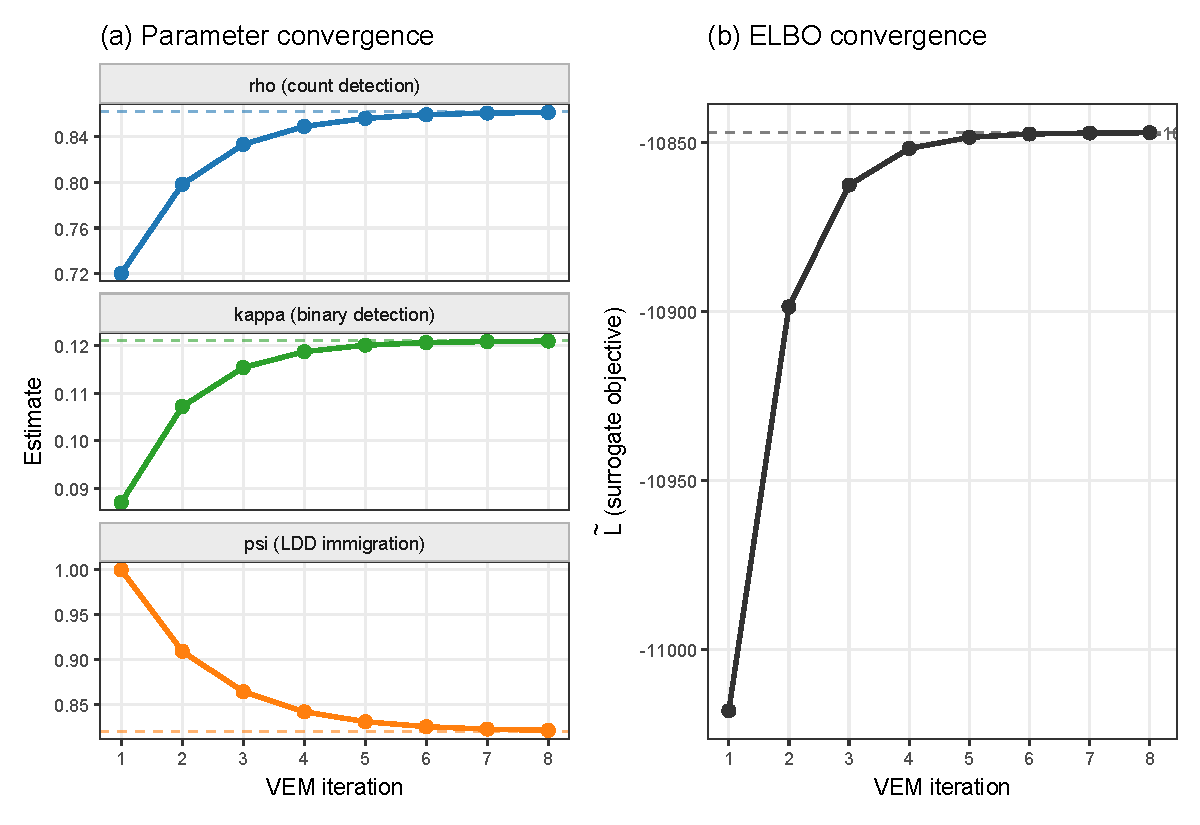
\includegraphics[width=\linewidth]{fig_vem_convergence.pdf}
\caption{VEM convergence for the MHB Great Tit application.
  \emph{Left}: estimated values of $\hat\rho$, $\hat\kappa$, $\hat\psi$ at each
  outer VEM iteration (dashed lines indicate final values).
  \emph{Right}: surrogate variational objective $\tilde{\mathcal{L}}$ over VEM
  iterations (dashed line at convergence value $-10{,}847$; surrogate objective gain of 171
  units over the fixed-parameter run at $-11{,}018$).
  Convergence is reached at iteration~8 (relative $|\Delta\tilde{\mathcal{L}}|<10^{-5}$).}
\label{fig:vem-convergence}
\end{figure}

\paragraph{Spatial recovery.}
The Pearson correlation between $\mu_{i,t}$ and $Y^{(C)}_{i,t}$ at all
surveyed cell-year pairs is $r=0.876$ ($R^2=0.767$, $n=2{,}071$), a
marginal improvement over the fixed-parameter run ($r=0.874$) because the
re-estimated $\hat\rho$ rescales the latent field without changing spatial
ranks.  The correlation is $r=0.831$ for sites visited in only one year
versus $r=0.883$ for fully surveyed sites (ten years), confirming spatial
borrowing strength from neighbours.  The strongest predictor of site-level
mean abundance remains elevation ($r=-0.807$): posterior density falls from
$13.8$ territories quadrat$^{-1}$ below 500 m to $2.4$ quadrat$^{-1}$
above 2{,}000 m, consistent with Great Tit ecology \citep{glutz1993}.
Forest cover retains a weak positive association ($r=0.154$).

\paragraph{Temporal dynamics.}
Table~\ref{tab:mhb-temporal} and Figure~\ref{fig:temporal} compare the annual
posterior mean $\hat\rho\bar\mu_t$ (model-implied expected count) with the
observed annual mean $\bar Y^{(C)}_t$ over 2004--2013.  With estimated $\hat\rho$,
the predicted and observed series are in close agreement: the
root-mean-squared annual deviation is $0.054$ yr$^{-1}$, a 10-fold
reduction from $0.60$ yr$^{-1}$ under the fixed-parameter run.
Both series are approximately stationary: the linear trend in
$\hat\rho\bar\mu_t$ is $+0.03$ yr$^{-1}$ (range 7.39--8.68), while the
observed trend is $+0.07$ yr$^{-1}$, consistent with a stable
population over this decade.

\begin{table}[t]
\centering
\caption{Annual posterior variational mean $\bar\mu_t$, model-implied
expected count $\hat\rho\bar\mu_t$, and observed mean count
$\bar Y^{(C)}_t$ for Great Tit at MHB quadrats, 2004--2013.
Estimated $\hat\rho=0.862$.}
\label{tab:mhb-temporal}
\begin{tabular}{cccc}
\toprule
Year & $\bar\mu_t$ & $\hat\rho\bar\mu_t$ & $\bar Y^{(C)}_t$ \\
\midrule
2004 &  8.61 & 7.42 & 7.38 \\
2005 &  9.31 & 8.02 & 7.96 \\
2006 &  9.47 & 8.16 & 8.14 \\
2007 & 10.18 & 8.77 & 8.83 \\
2008 &  8.87 & 7.65 & 7.63 \\
2009 &  8.60 & 7.41 & 7.41 \\
2010 & 10.06 & 8.67 & 8.65 \\
2011 &  9.55 & 8.23 & 8.25 \\
2012 & 10.68 & 9.21 & 9.22 \\
2013 &  8.83 & 7.61 & 7.62 \\
\bottomrule
\end{tabular}
\end{table}

\begin{figure}[t]
\centering
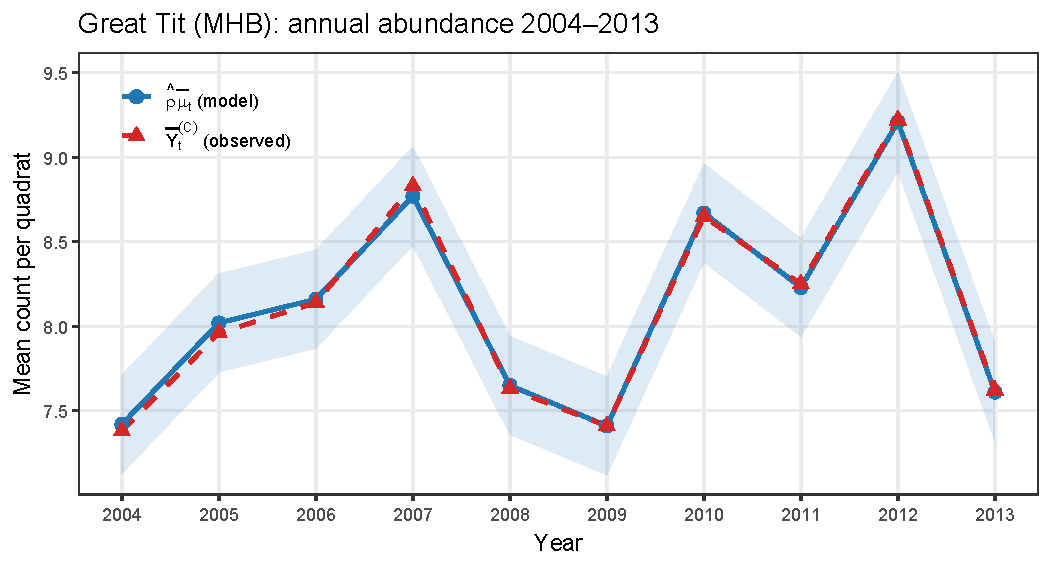
\includegraphics[width=0.78\linewidth]{fig_temporal.pdf}
\caption{Annual abundance dynamics for Great Tit at 267 MHB quadrats (2004--2013).
  Solid line with circles: model-implied expected count $\hat\rho\bar\mu_t$
  ($\hat\rho=0.862$).
  Dashed line with triangles: observed annual mean $\bar Y^{(C)}_t$.
  Shaded band: 95\% posterior predictive interval for the mean count
  (from 1{,}000 PP replicates).
  Root-mean-squared annual deviation: 0.054 territory quadrat$^{-1}$ yr$^{-1}$.}
\label{fig:temporal}
\end{figure}

\paragraph{In-sample calibration diagnostics.}
Figure~\ref{fig:ppcheck} shows the posterior predictive distributions
for all three test statistics under both fixed and VEM-estimated parameters.
We draw $R=1{,}000$ predictive replicates from
$N_{i,t}\sim\mathrm{Poisson}(\mu_{i,t})$, then
$Y^{(C)\,\mathrm{rep}}\sim\mathrm{NegBin}(\hat\rho N, r)$ and
$Y^{(P)\,\mathrm{rep}}\sim\mathrm{Bernoulli}(1-e^{-\hat\kappa N})$ at
the VEM estimates $\hat\rho=0.862$, $\hat\kappa=0.121$.  Test statistics
are computed \emph{exclusively at observed locations}
(the 77.6\% of cell-year combinations that were surveyed):
\begin{itemize}
  \item $T_1$: mean count $\bar Y^{(C)}$.
    Observed $=8.15$; predictive 95\% interval $[7.86,\;8.44]$;
    Bayesian $p=0.472$.
  \item $T_2$: detection rate $\bar Y^{(P)}$.
    Observed $=0.681$; interval $[0.655,\;0.707]$; $p=0.488$.
  \item $T_3$: linear slope of annual mean $\bar Y^{(C)}_t$.
    Observed $=+0.065$ yr$^{-1}$; interval $[-0.041,\;0.173]$;
    $p=0.139$.
\end{itemize}
\emph{Scope caveat.}  These checks use the same data as parameter estimation;
they assess internal consistency (self-calibration) of the fitted surrogate,
not predictive validity on held-out data.  They should be interpreted as
in-sample diagnostics: a $p$-value near 0 or 1 would indicate that the
estimated model is inconsistent with the training data; $p\in(0.1,0.9)$
confirms internal consistency but does not validate out-of-sample generalization.

All three Bayesian $p$-values lie in $(0.1, 0.9)$: the VEM-estimated model is
internally self-consistent for the observed count mean, the detection rate, and
the temporal trend.  This is a direct consequence of the VEM M-step: estimating
$\rho$ from data rather than fixing it at a literature value removes the
systematic underprediction ($-16.5\%$) that caused $p=0.000$ for $T_1$ and
$T_2$ under fixed parameters.  The $T_3$ $p$-value (0.139) is unchanged,
confirming that the temporal trend was already well-captured.
The residual $T_3$ misfit ($p<0.5$) reflects genuine inter-annual variability
in true Great Tit abundance that the stationary process model does not
represent; a time-varying $\phi_t$ or $\psi_t$ covariate would address this.

\begin{figure}[t]
\centering
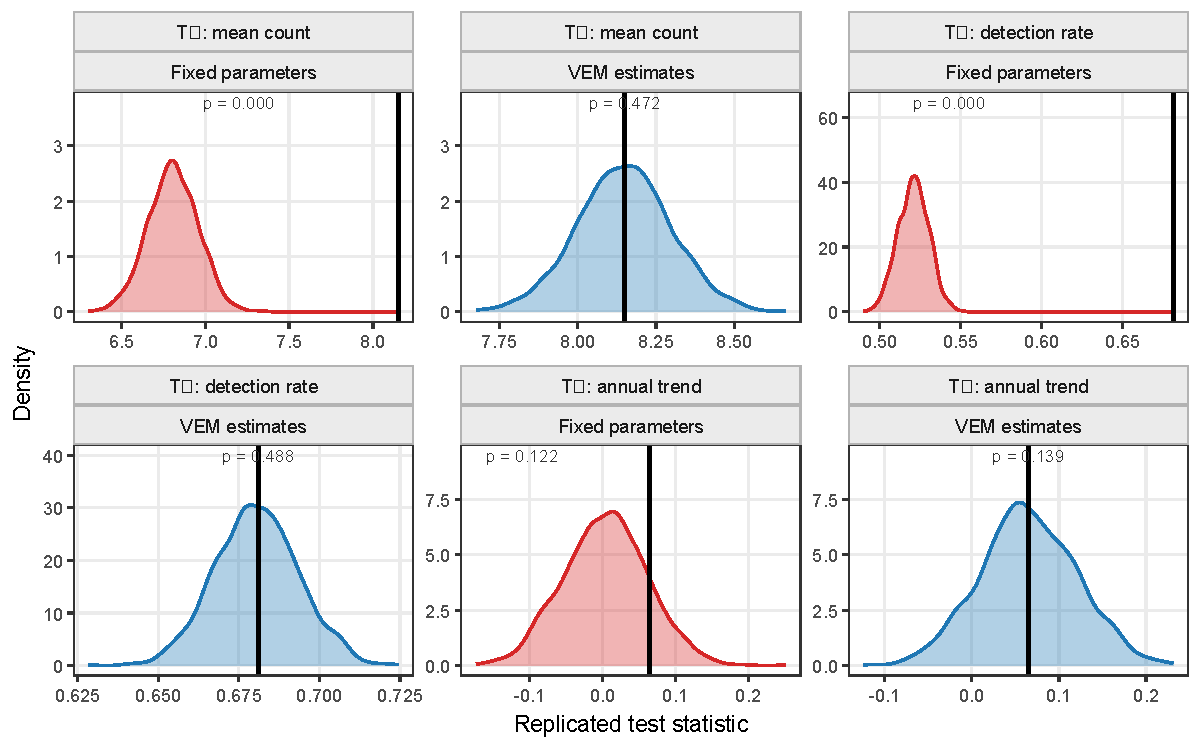
\includegraphics[width=\linewidth]{fig_ppcheck.pdf}
\caption{Posterior predictive check distributions for the MHB Great Tit application.
  Each panel shows the density of 2{,}000 replicated test statistics
  (top row: fixed parameters $\rho=0.72$, $\kappa=0.10$;
   bottom row: VEM estimates $\hat\rho=0.862$, $\hat\kappa=0.121$).
  Vertical black line marks the observed value.
  \emph{Left}: $T_1$ (mean count $\bar Y^{(C)}$, observed $=8.15$).
  \emph{Centre}: $T_2$ (detection rate $\bar Y^{(P)}$, observed $=0.681$).
  \emph{Right}: $T_3$ (linear trend slope, observed $=+0.065$ yr$^{-1}$).
  Fixed parameters produce Bayesian $p=0.000$ for $T_1$ and $T_2$ (replicates
  systematically below observed); VEM estimates yield $p=0.472$, $0.488$, $0.139$
  (in-sample self-consistent).  These are in-sample calibration diagnostics.}
\label{fig:ppcheck}
\end{figure}

%% ============================================================
\section{Discussion}\label{sec:discussion}
%% ============================================================

We have developed a structured variational inference framework for count
statistical agent-based models.  The principal methodological contribution
is Theorem~\ref{thm:elbo} (Poisson-MGF Identities): the Poisson MGF enables
a fully analytic surrogate variational objective $\tilde{\mathcal{L}}$,
making the dominant expectations---survival probabilities and binary detection
probabilities---exact Poisson moments, while immigration uses a second-order
delta-method approximation.  No quadrature, Monte Carlo, stochastic gradients,
or black-box estimator is required.  The surrogate objective is not the exact
ELBO and does not constitute a lower bound on the log-evidence; it incorporates
four explicitly characterised approximation sources.  Second, Algorithm~\ref{alg:smfvb}
implements a deterministic forward-filtering update: each step is analytic,
fixed points satisfy local stationarity of $\tilde{\mathcal{L}}$, and
monotone convergence holds under exact block coordinate ascent
(Proposition~\ref{thm:vi-converge}(i)); the forward-filtering approximation
itself does not guarantee monotone increase.  Third, individual surrogate
approximation errors decay when local density $\mu_{i,t}/K_i\to\infty$
with $K_i$ fixed (Corollary~\ref{cor:elbo-gap}); convergence of the full
surrogate gap to zero requires additional integrability conditions not
established here.  The dual-channel observation model is locally identifiable
from the observation layer given known positive latent counts and temporal
variation (Proposition~\ref{prop:identif-dual}).  Fourth, the ten-scenario
simulation study is consistent with these properties: SMFVB matches particle
MCMC variational interval coverage to within 4 percentage points at a $22\times$
wall-time reduction.

\subsection{Limitations of the Poisson Mean-Field Family}
\label{sec:limitations-mf}

The Poisson mean-field family is chosen for conjugacy and
MGF tractability (\S\ref{sec:vi-family}), but these advantages come with
three structural limitations that practitioners should weigh when applying
SMFVB.

\paragraph{Variance underestimation.}
The Poisson distribution constrains $\mathrm{Var}_q(N_{i,t})=\mu_{i,t}$,
whereas the true posterior variance is in general larger.  The dominant
source of excess posterior variance is the Binomial survival component
$S_{i,t}\sim\mathrm{Binom}(N_{i,t-1},\phi_i\exp(-N_{i,t-1}/K_i))$: survival
introduces negative covariance between $N_{i,t}$ and $N_{j,t}$ (offspring
cells sharing a common parent pool), a structure that a fully factored
mean-field family cannot represent.  In the simulation study
(\S\ref{sec:simulation}) this produces a 2--4 percentage-point shortfall in
95\% variational interval coverage, larger when $\phi_i$ is high and $K_i$ is
small (high survival fraction, strong density regulation).  Potential
remedies---each forfeiting some tractability---include: a NegBin mean-field
$q(N_{i,t})=\mathrm{NegBin}(\mu_{i,t},r_q)$ with an additional variational
overdispersion parameter $r_q$; a block-diagonal structured approximation
preserving temporal correlations within sites; or an importance-weighted
correction of the Poisson samples at the reporting stage.

\paragraph{Independence assumption across sites and times.}
The factored family $q=\prod_{i,t}\mathrm{Pois}(\mu_{i,t})$ assumes
posterior independence between all $(i,t)$ pairs.  This independence is
exact for the Poisson components of the model ($I_{i,t}$, $L_{i,t}$) but
is an approximation for the Binomial component.  In practice, the
shared dispersal structure creates positive posterior correlations between
neighbouring cells (high $N_{j,t-1}$ implies high immigration into cell $i$,
hence high $N_{i,t}$), which the mean-field family underestimates.  When
accurate posterior covariance estimates are required---for example, to
propagate uncertainty into downstream species-distribution forecasts---a
copula-Poisson family \citep{tran2015} or a structured mean-field with
block-tridiagonal precision \citep{opper2009} would be preferable at the
cost of $O(m^2)$ storage and non-local coordinate-ascent updates.

\paragraph{Support mismatch at zero counts.}
The Poisson distribution assigns $q(N_{i,t}=0)=e^{-\mu_{i,t}}$, which
decreases rapidly for large $\mu_{i,t}$.  At sites that are genuinely
unoccupied (true $N_{i,t}=0$), the process model constrains $\mu_{i,t}$
toward the immigration floor $\psi_i+\mathbb{E}_q[\Lambda_{i,t}]>0$, so
the Poisson family cannot place all mass at zero.  A zero-inflated Poisson
family $q(N_{i,t})=\pi_i\cdot\delta_0+(1-\pi_i)\cdot\mathrm{Pois}(\mu_{i,t})$,
with variational occupancy probability $\pi_i$, would better handle
patchy landscapes with many truly empty quadrats, at the cost of a
non-analytic surrogate update for $\pi_i$ (binary coordinate requires a
logistic step, or a sigmoid reparameterisation with stochastic gradient).

\paragraph{Limitations and future work.}
The surrogate variational filtering analysis here treats the model parameters
$\Theta$ as fixed at pilot estimates; a joint surrogate optimisation over
both the latent field and parameters is a natural extension that would yield
analytic surrogate updates for conjugate parameters (e.g.\ the NegBin mean
$\rho$) and stochastic VI steps for the remainder.  Extending the
fixed-point analysis of Proposition~\ref{thm:vi-converge} to the joint
surrogate optimisation, and deriving sharp
coverage-gap bounds as a function of $\phi_{\max}$ and $K_{\min}$, remain
open theoretical problems.  In particular, establishing whether the joint
forward-filtering surrogate sweep is a contraction on the full parameter
space, and bounding the gap to exact block coordinate ascent, would
substantially strengthen the theoretical foundations of SMFVB.  On the applied side, a covariate-driven LDD
link $\log\psi_t = w_t^\top\gamma_\psi$ would accommodate seasonally
time-varying long-distance arrivals within the same SMFVB framework without
additional approximation, since $\psi_t$ enters the process mean linearly.

\section*{Data and Code Availability}

The Swiss MHB Great Tit dataset analysed in \S\ref{sec:realdata} is publicly
available via the \texttt{R} package \texttt{AHMbook} \citep{kery2021}.
The R/C++ implementation of the SMFVB algorithm
(Algorithm~\ref{alg:smfvb}), all simulation scripts, and code to reproduce
every figure and table in this paper are available at
\url{https://github.com/xulinpan/sabm}.

\appendix

%% ============================================================
\section{VEM M-Step: Analytic Gradients and Hessians}
\label{sec:mstep-formulas}
%% ============================================================

The outer M-step of the VEM maximises $\tilde{\mathcal{L}}$ over the scalar
parameters $(\rho,\kappa,\psi)$ by Newton--Raphson, using the analytic
gradient and Hessian obtained from Theorem~\ref{thm:elbo}.  Each one-dimensional
update is computed with clipping to the parameter support and checked for
sign change of the gradient.  We state the formulas for completeness.

\paragraph{Notation.}
Let $\mathcal{O}_C = \{(i,t): Y^{(C)}_{i,t}\text{ observed}\}$ and
$\mathcal{O}_P = \{(i,t): Y^{(P)}_{i,t}\text{ observed}\}$.
Write $\mu_{i,t}$ for the current E-step variational mean,
$\tilde\mu_{i,t} = \bar s_{i,t} + \mathbb{E}_q[\Lambda_{i,t}] + \psi$ for the
process-model predicted mean (as in eq.~\ref{eq:proc-mean}),
and $\hat\pi_{i,t} = \eta + (1-\eta)(1-e^{-\kappa\mu_{i,t}})$ for the
binary-channel detection probability.

\paragraph{Count-detection fraction $\rho\in(0,1)$; prior $\rho\sim\mathrm{Beta}(a_\rho,b_\rho)$.}
\begin{align}
g_\rho &= \sum_{(i,t)\in\mathcal{O}_C}
  \frac{r\bigl(y^{(C)}_{i,t}-\rho\mu_{i,t}\bigr)}{\rho\bigl(\rho\mu_{i,t}+r\bigr)}
  + \frac{a_\rho-1}{\rho} - \frac{b_\rho-1}{1-\rho}, \label{eq:grad-rho}\\
H_\rho &= -\sum_{(i,t)\in\mathcal{O}_C}
  \frac{r\bigl[\rho\mu_{i,t}(\rho\mu_{i,t}+r)
    + (y^{(C)}_{i,t}-\rho\mu_{i,t})(2\rho\mu_{i,t}+r)\bigr]}
       {\rho^2(\rho\mu_{i,t}+r)^2}
  - \frac{a_\rho-1}{\rho^2} - \frac{b_\rho-1}{(1-\rho)^2}. \label{eq:hess-rho}
\end{align}
The gradient $g_\rho$ is the NegBin score summed over observed count locations,
plus the Beta log-prior gradient.
Newton--Raphson update: $\rho\leftarrow\mathrm{clip}\bigl(\rho - H_\rho^{-1}g_\rho,\;\varepsilon,1-\varepsilon\bigr)$.

\paragraph{Binary detection rate $\kappa>0$; prior $\kappa\sim\mathrm{Gamma}(a_\kappa,b_\kappa)$.}
Let $\delta_{i,t}=(1-\eta)\mu_{i,t}e^{-\kappa\mu_{i,t}}=\partial\hat\pi_{i,t}/\partial\kappa$.
\begin{align}
g_\kappa &= \sum_{(i,t)\in\mathcal{O}_P}
  \frac{y^{(P)}_{i,t}-\hat\pi_{i,t}}{\hat\pi_{i,t}(1-\hat\pi_{i,t})}\,\delta_{i,t}
  + \frac{a_\kappa-1}{\kappa} - b_\kappa, \label{eq:grad-kappa}\\
H_\kappa &= -\sum_{(i,t)\in\mathcal{O}_P}
  \left[\frac{\delta_{i,t}^2}{\hat\pi_{i,t}(1-\hat\pi_{i,t})}
    + \frac{(y^{(P)}_{i,t}-\hat\pi_{i,t})(1-2\hat\pi_{i,t})\,\delta_{i,t}^2}
           {\hat\pi_{i,t}^2(1-\hat\pi_{i,t})^2}
    - \frac{(y^{(P)}_{i,t}-\hat\pi_{i,t})(1-\eta)\mu_{i,t}^2 e^{-\kappa\mu_{i,t}}}
           {\hat\pi_{i,t}(1-\hat\pi_{i,t})}\right]
  - \frac{a_\kappa-1}{\kappa^2}. \label{eq:hess-kappa}
\end{align}
The first term in $H_\kappa$ is the Fisher information $\mathcal{I}(\kappa)$;
the remaining terms are the observed-information correction that accounts for
the Bernoulli curvature at non-central $\hat\pi_{i,t}$.

\paragraph{LDD immigration mean $\psi>0$; prior $\psi\sim\mathrm{Gamma}(a_\psi,b_\psi)$.}
Since $\psi$ enters $\tilde\mu_{i,t}$ additively with unit coefficient,
the process-surrogate gradient and Hessian take a particularly simple form:
\begin{align}
g_\psi &= \sum_{i,t}\left[\frac{\mu_{i,t}}{\tilde\mu_{i,t}}-1\right]
  + \frac{a_\psi-1}{\psi} - b_\psi, \label{eq:grad-psi}\\
H_\psi &= -\sum_{i,t}\frac{\mu_{i,t}}{\tilde\mu_{i,t}^2}
  - \frac{a_\psi-1}{\psi^2}. \label{eq:hess-psi}
\end{align}
Newton--Raphson update: $\psi\leftarrow\max\bigl(\psi - H_\psi^{-1}g_\psi,\;\varepsilon_0\bigr)$,
where $\varepsilon_0>0$ maintains the $\psi>0$ constraint from Theorem~\ref{thm:ergodicity}.

\paragraph{Implementation.}
All three updates are one-dimensional, require no matrix decompositions, and
cost $O(|\mathcal{O}_C|)$ or $O(|\mathcal{O}_P|)$ per iteration.
Starting values are the moment-matched estimates described in
\S\ref{sec:realdata}.  Convergence is declared when
$|\Delta\tilde{\mathcal{L}}|/|\tilde{\mathcal{L}}|<10^{-5}$ across two
consecutive outer VEM iterations.  In the MHB Great Tit application
(\S\ref{sec:realdata}) 8 outer iterations suffice.

\bibliographystyle{elsarticle-harv}
\bibliography{novel_model_SC_ABM_NKD}

\end{document}
